% !TeX root = ../main.tex

\subsubsection{載台部分}

本系統的載台設計遵循「由下往上」的堆疊邏輯，依序為 X 軸、Y 軸、Z 軸，最後為最頂層的樣本夾持機構。

X 軸馬達座 (X\_Motor\_Mount)：用於將 NEMA 17 步進馬達穩固地固定於 X 軸傳動鏈的起點。此座體透過多點卡合於框架上，為馬達提供穩固支撐，確保馬達軸心與 T8 螺桿始終維持良好的同軸度。

X 軸軸承座 (X\_Bearing\_Mount)：安裝於 X 軸 T8 螺桿的末端，內部可容納一組軸承。此部件的主要功能是為高速旋轉的螺桿提供徑向支撐，減少長螺桿在高速旋轉時可能產生的偏擺（Whiplash）現象，從而提升 X 軸掃描時的定位精度。

X 軸被動端支架 (X\_Driven\_Bracket)：作為 X 軸傳動機構被動端的結構支撐。此部件並不直接與 X 軸軸承座緊密配合，而是透過 Y 軸至 X 軸轉接件同步 X 軸的位置，作為螺桿遠端的懸空支撐點，以維持整個 X 軸傳動系統的結構穩定性。

X 軸 T8 螺帽支架 (X\_T8\_Nut\_Bracket)：用於牢固包裹並鎖緊 T8 黃銅螺帽，並與移動滑塊進行連接。此部件負責將 T8 螺桿的旋轉運動轉換為 X 軸方向的線性平移，是整個 X 軸動力傳遞的核心元件。

X 軸導軌樂高轉接件 (X\_Rail\_Lego\_Adapter)：是實現「樂高結構」與「工業級線性滑軌」無縫接合的關鍵介面。此轉接件頂部設有與金屬滑軌相容的沉頭螺栓孔，底部則帶有標準的樂高插銷陣列，成功將工業級的平滑運動特性引入了樂高搭建的低成本框架中。

X 軸導軌至軸承轉接件 (X\_Rail\_To\_Bearing\_Adapter)：搭載於 X 軸導軌樂高轉接件 (X\_Rail\_Lego\_Adapter) 上。此轉接件的固定螺孔設計為可前後輕易調整位置的長形孔，使安裝時能彈性補償 3D 列印公差。

\begin{figure}[H]
    \centering
    \begin{minipage}[b]{0.48\textwidth}
        \centering
        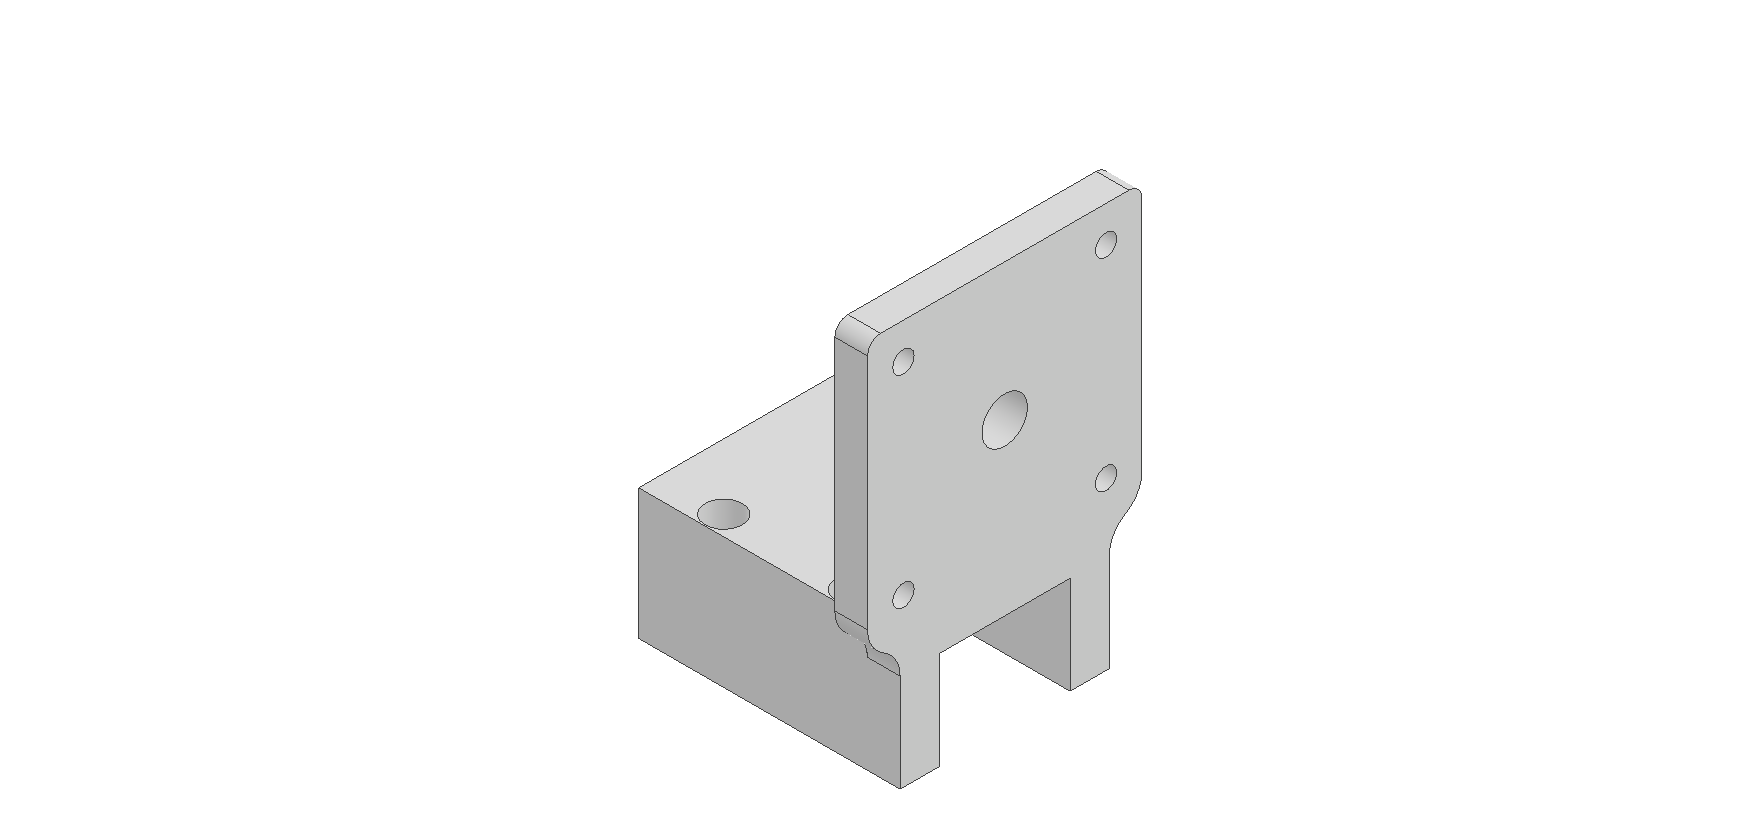
\includegraphics[width=\textwidth]{figures/ch3/fig3_21_a_X_Motor_Mount.png}
        \par (a) X 軸馬達座
    \end{minipage}
    \hfill
    \begin{minipage}[b]{0.48\textwidth}
        \centering
        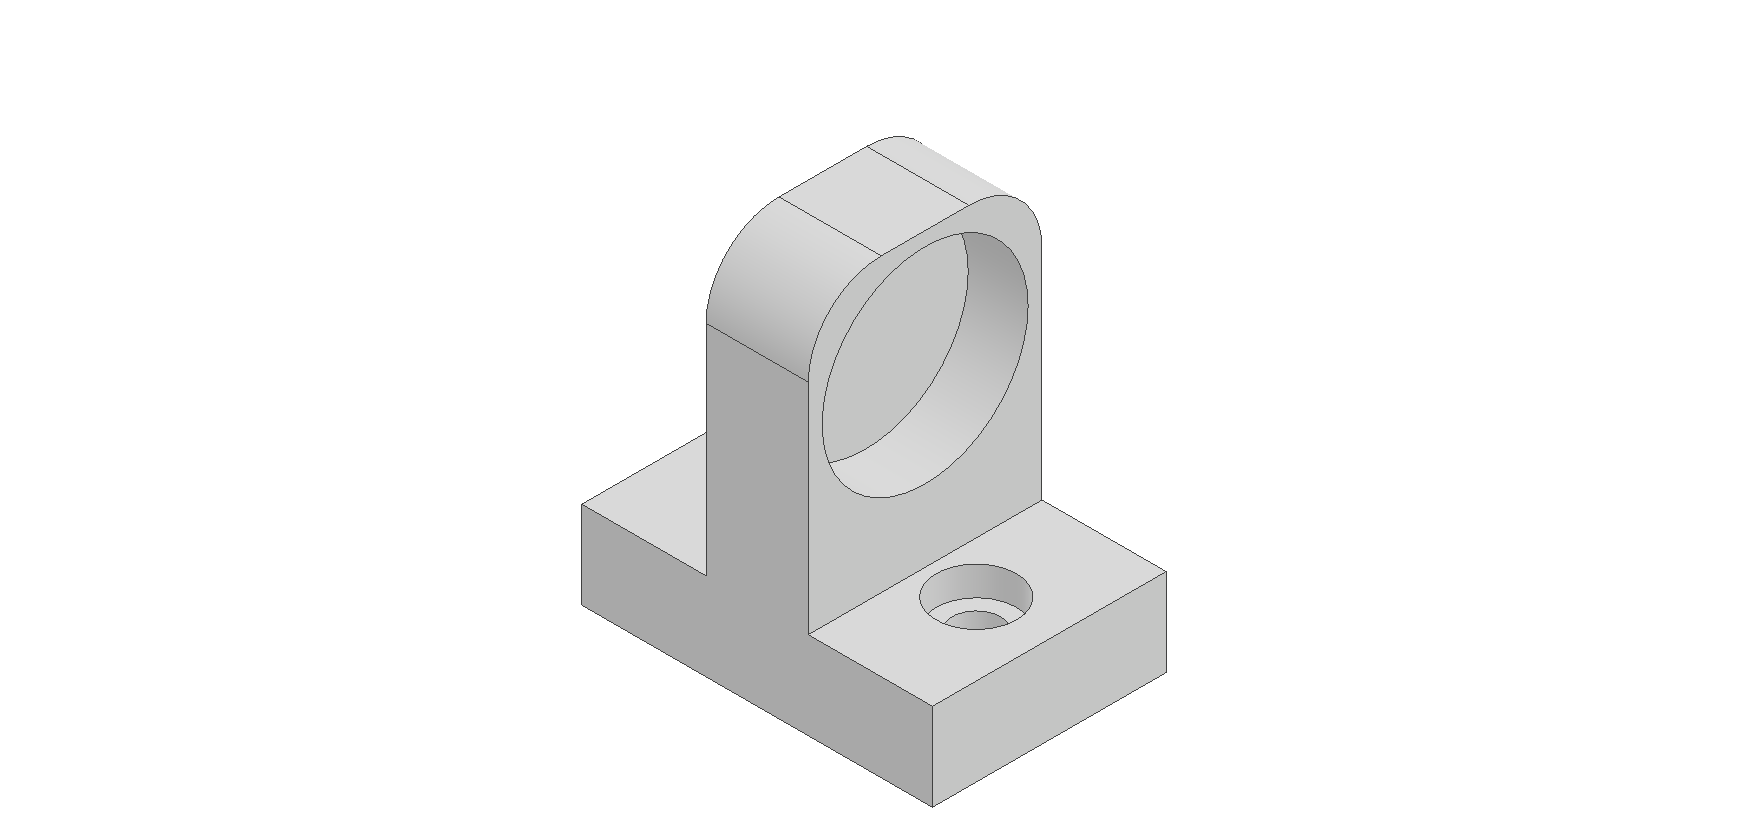
\includegraphics[width=\textwidth]{figures/ch3/fig3_21_b_X_Bearing_Mount.png}
        \par (b) X 軸軸承座
    \end{minipage}
    \vspace{0.5cm}
    \begin{minipage}[b]{0.48\textwidth}
        \centering
        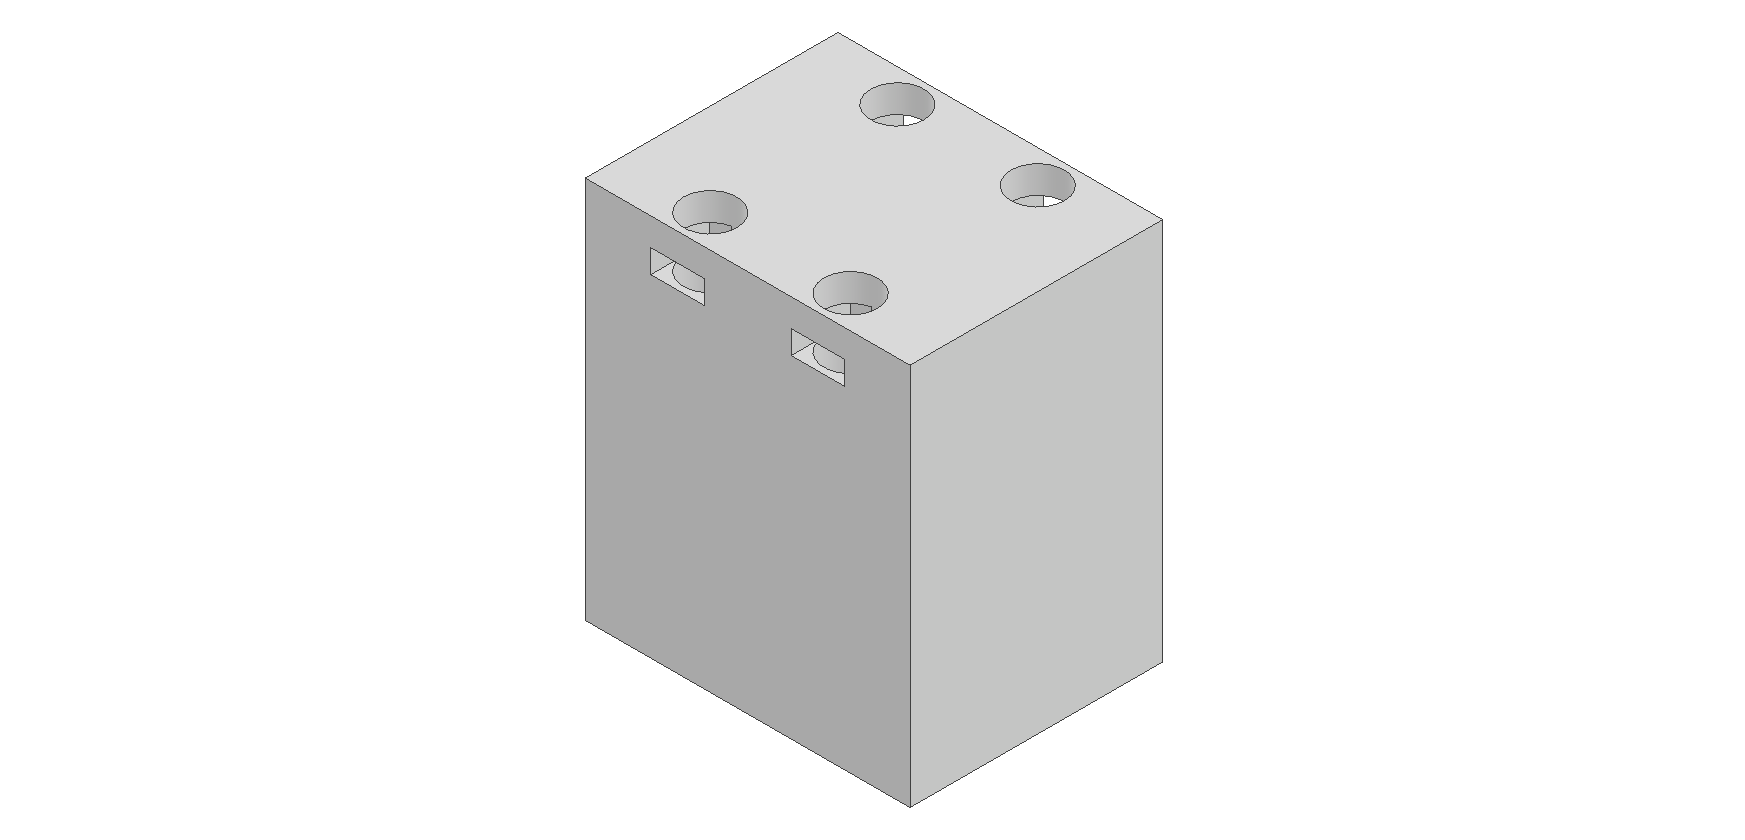
\includegraphics[width=\textwidth]{figures/ch3/fig3_21_c_X_Driven_Bracket.png}
        \par (c) X 軸被動端支架
    \end{minipage}
    \hfill
    \begin{minipage}[b]{0.48\textwidth}
        \centering
        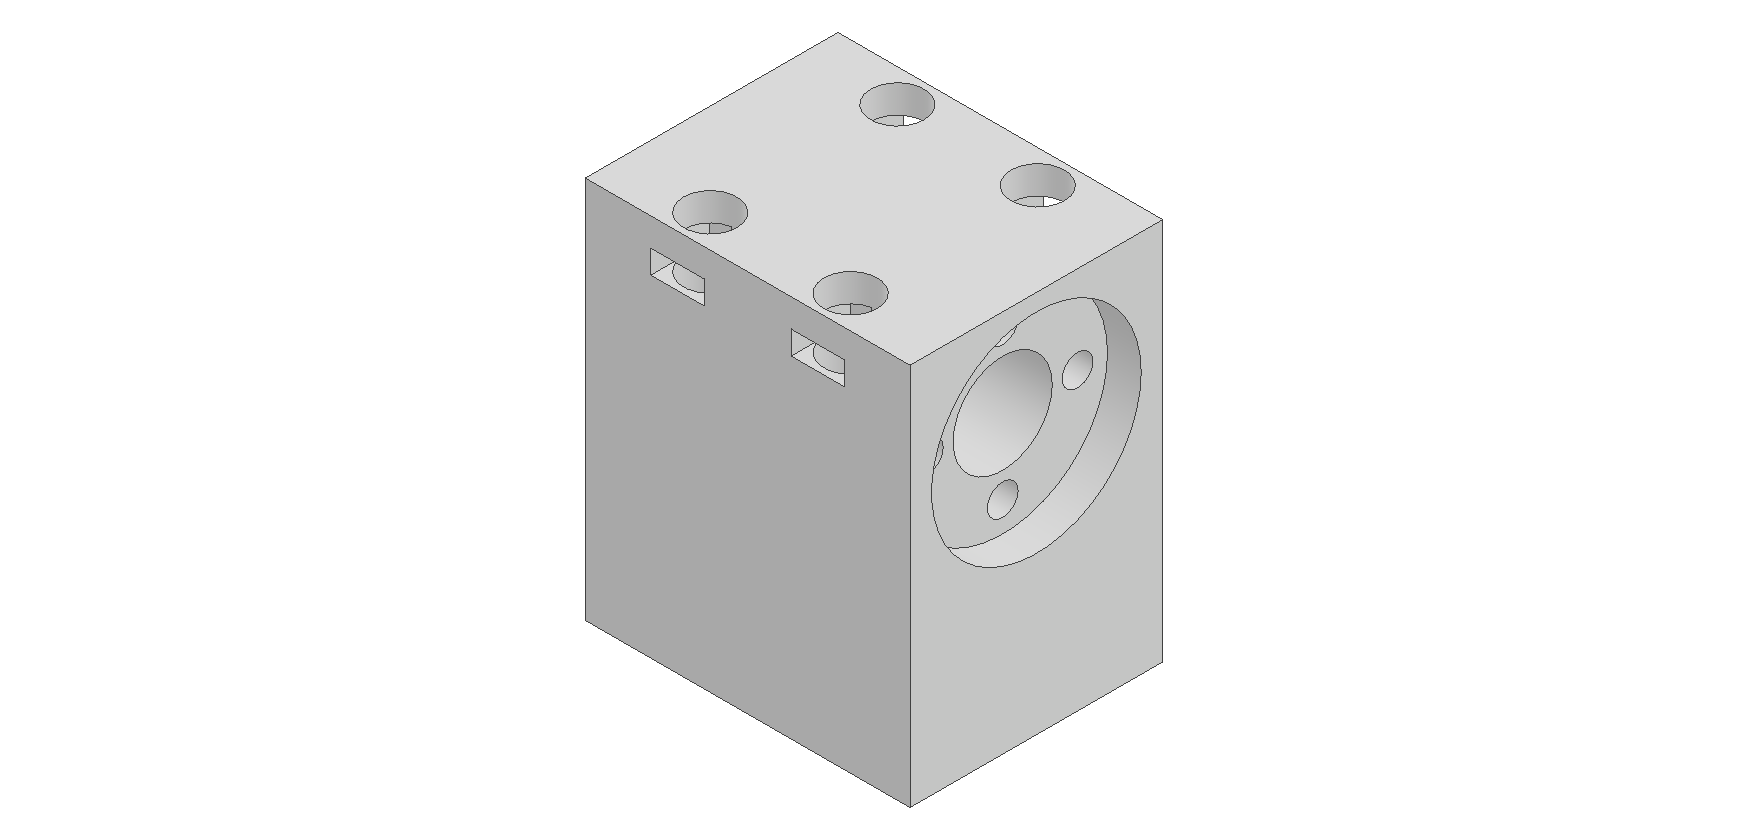
\includegraphics[width=\textwidth]{figures/ch3/fig3_21_d_X_T8_Nut_Bracket.png}
        \par (d) X 軸 T8 螺帽支架
    \end{minipage}
    \vspace{0.5cm}
    \begin{minipage}[b]{0.48\textwidth}
        \centering
        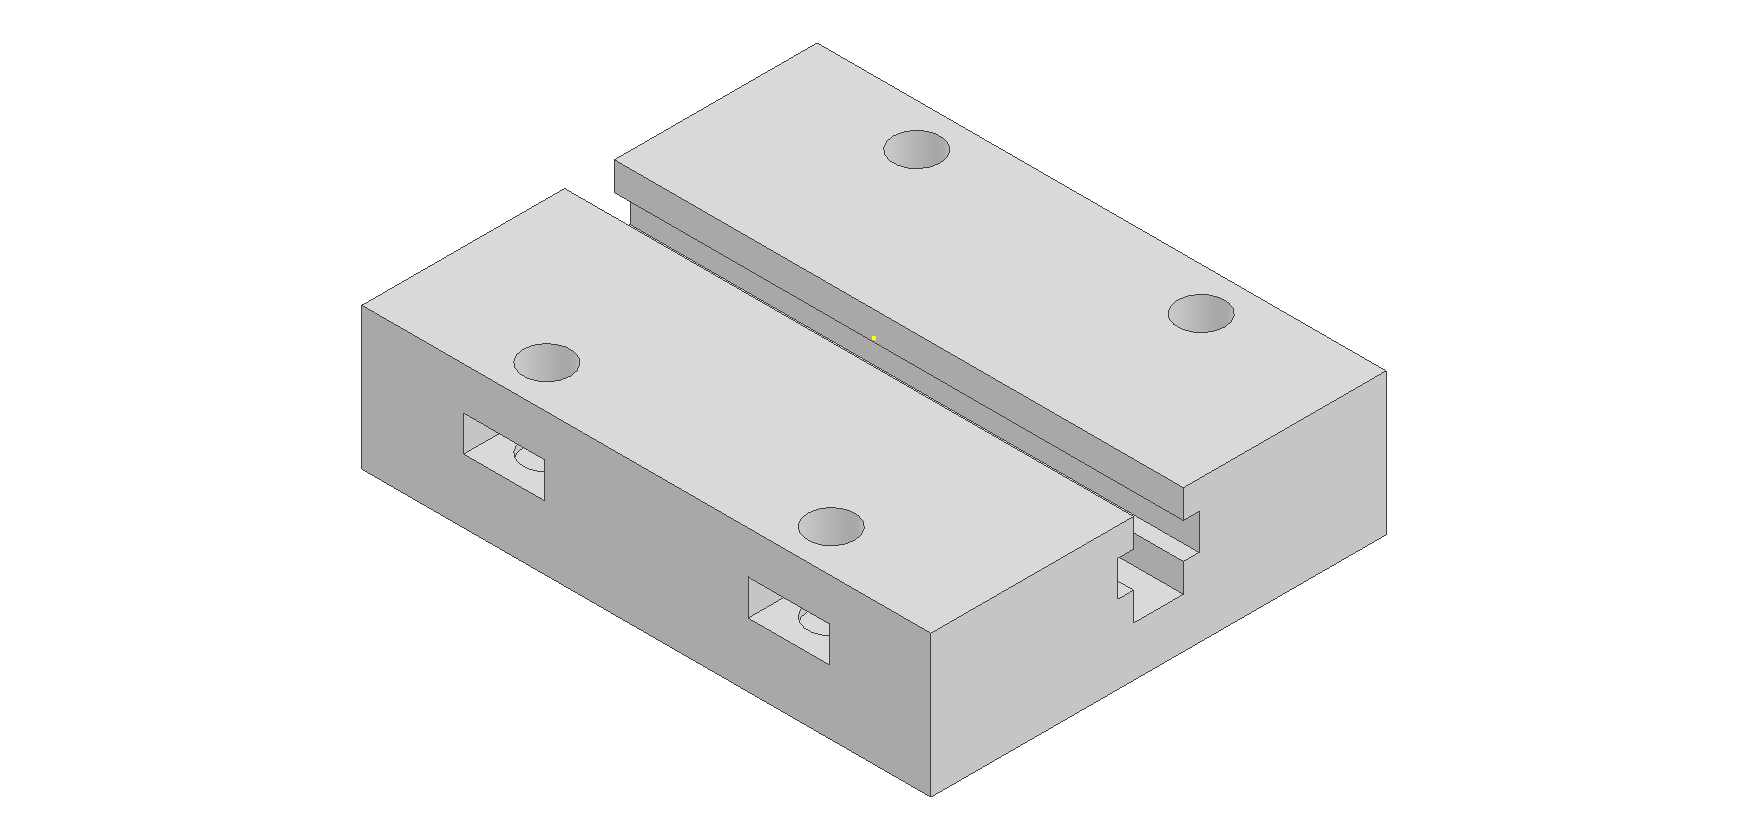
\includegraphics[width=\textwidth]{figures/ch3/fig3_21_e_X_Rail_Lego_Adapter.png}
        \par (e) X 軸導軌樂高轉接件
    \end{minipage}
    \hfill
    \begin{minipage}[b]{0.48\textwidth}
        \centering
        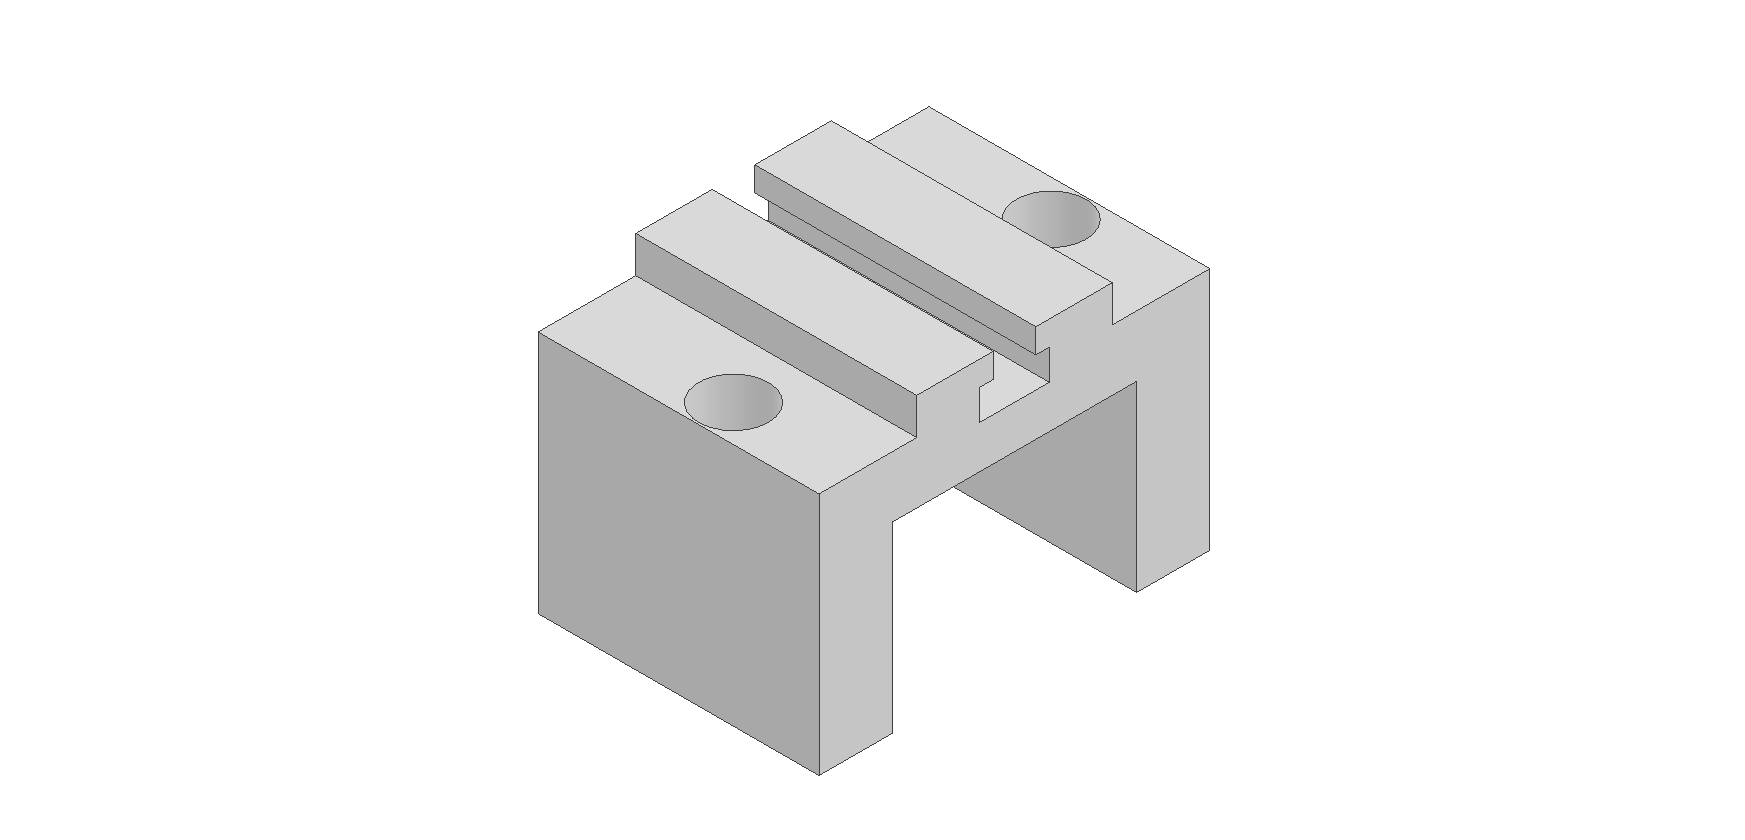
\includegraphics[width=\textwidth]{figures/ch3/fig3_21_f_X_Rail_To_Bearing_Adapter.png}
        \par (f) X 軸導軌至軸承轉接件
    \end{minipage}
    \caption{X 軸部件}
    \label{fig:stage_x}
\end{figure}

Y 軸馬達座 (Y\_Motor\_Mount)：用於將 NEMA 17 步進馬達穩固地固定於 Y 軸傳動鏈的起點。此座體透過多點卡合於框架上，為馬達提供穩固支撐，確保馬達軸心與 T8 螺桿始終維持良好的同軸度。

Y 軸軸承座 (Y\_Bearing\_Mount)：安裝於 Y 軸 T8 螺桿的末端，內部可容納一組軸承。此部件的主要功能是為高速旋轉的螺桿提供徑向支撐，減少長螺桿在高速旋轉時可能產生的偏擺（Whiplash）現象，從而提升 Y 軸掃描時的定位精度。

Y 軸 T8 螺帽支架 (Y\_T8\_Nut\_Bracket)：用於牢固包裹並鎖緊 T8 黃銅螺帽，並與移動滑塊進行連接。此部件負責將 T8 螺桿的旋轉運動轉換為 Y 軸方向的線性平移，是整個 Y 軸動力傳遞的核心元件。

Y 軸導軌至軸承轉接件 (Y\_Rail\_To\_Bearing\_Adapter)：此轉接件的固定螺孔設計為可前後輕易調整位置的長形孔，使安裝時能彈性補償 3D 列印公差。

Y 軸至 X 軸轉接件 (Y\_Rail\_To\_X\_Adapter)：為連接 Y 軸移動滑塊與 X 軸整體傳動機構的橫樑。此部件呈現一字型的長方形平板設計，承受著 Y 軸的重量與動態載荷，是實現系統 X-Y 二維平面正交（Orthogonal）精準運動的關鍵力學節點。

\begin{figure}[H]
    \centering
    \begin{minipage}[b]{0.48\textwidth}
        \centering
        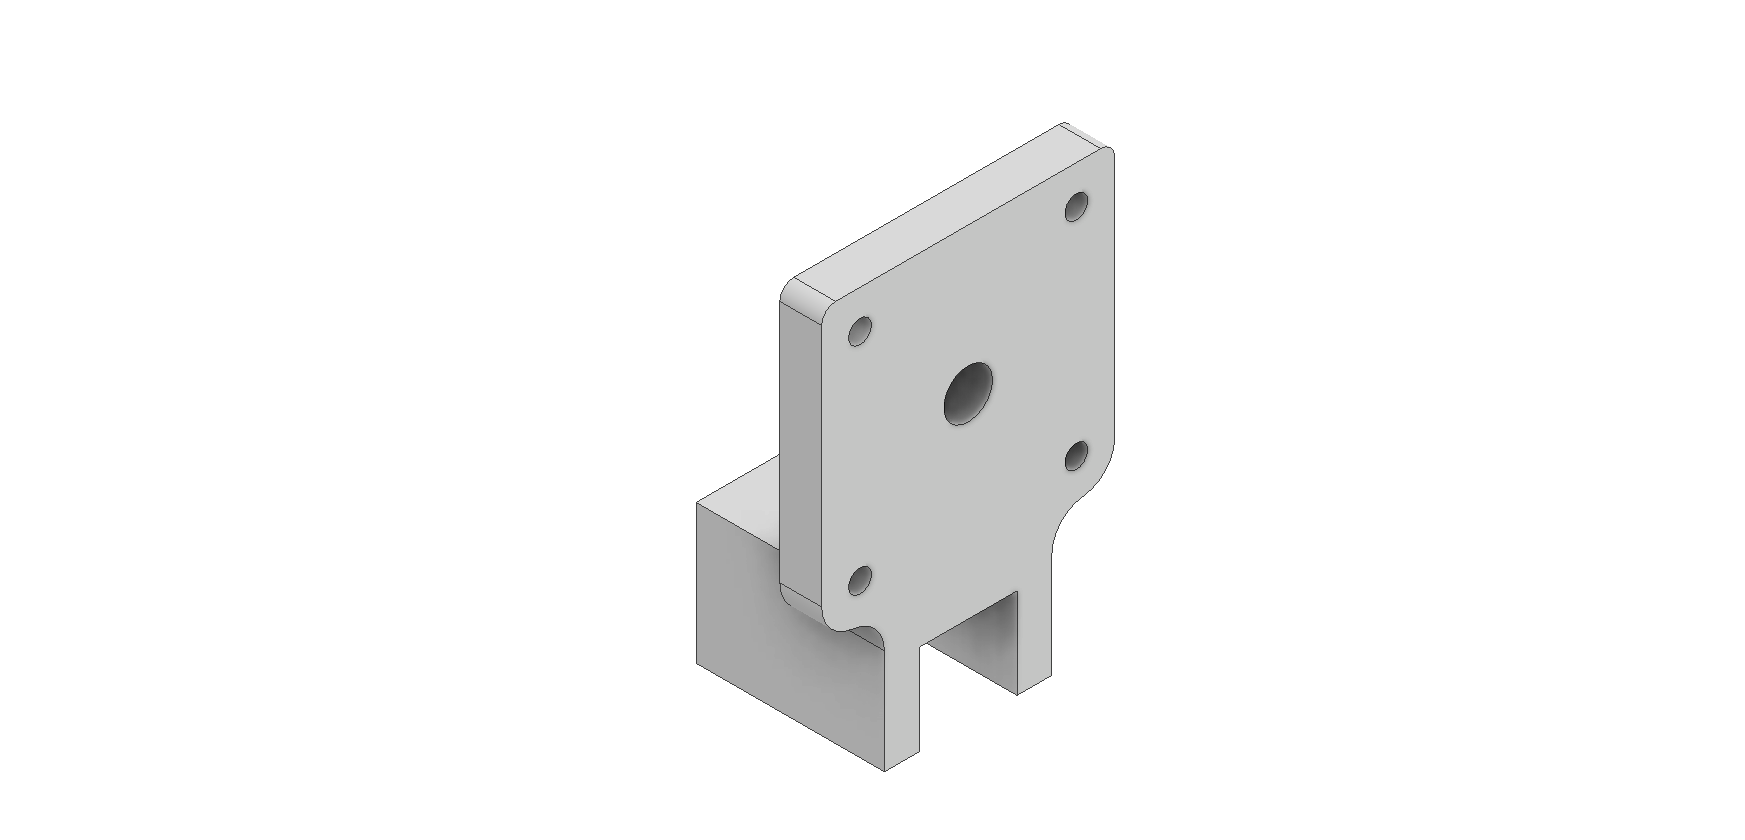
\includegraphics[width=\textwidth]{figures/ch3/fig3_22_a_Y_Motor_Mount.png}
        \par (a) Y 軸馬達座
    \end{minipage}
    \hfill
    \begin{minipage}[b]{0.48\textwidth}
        \centering
        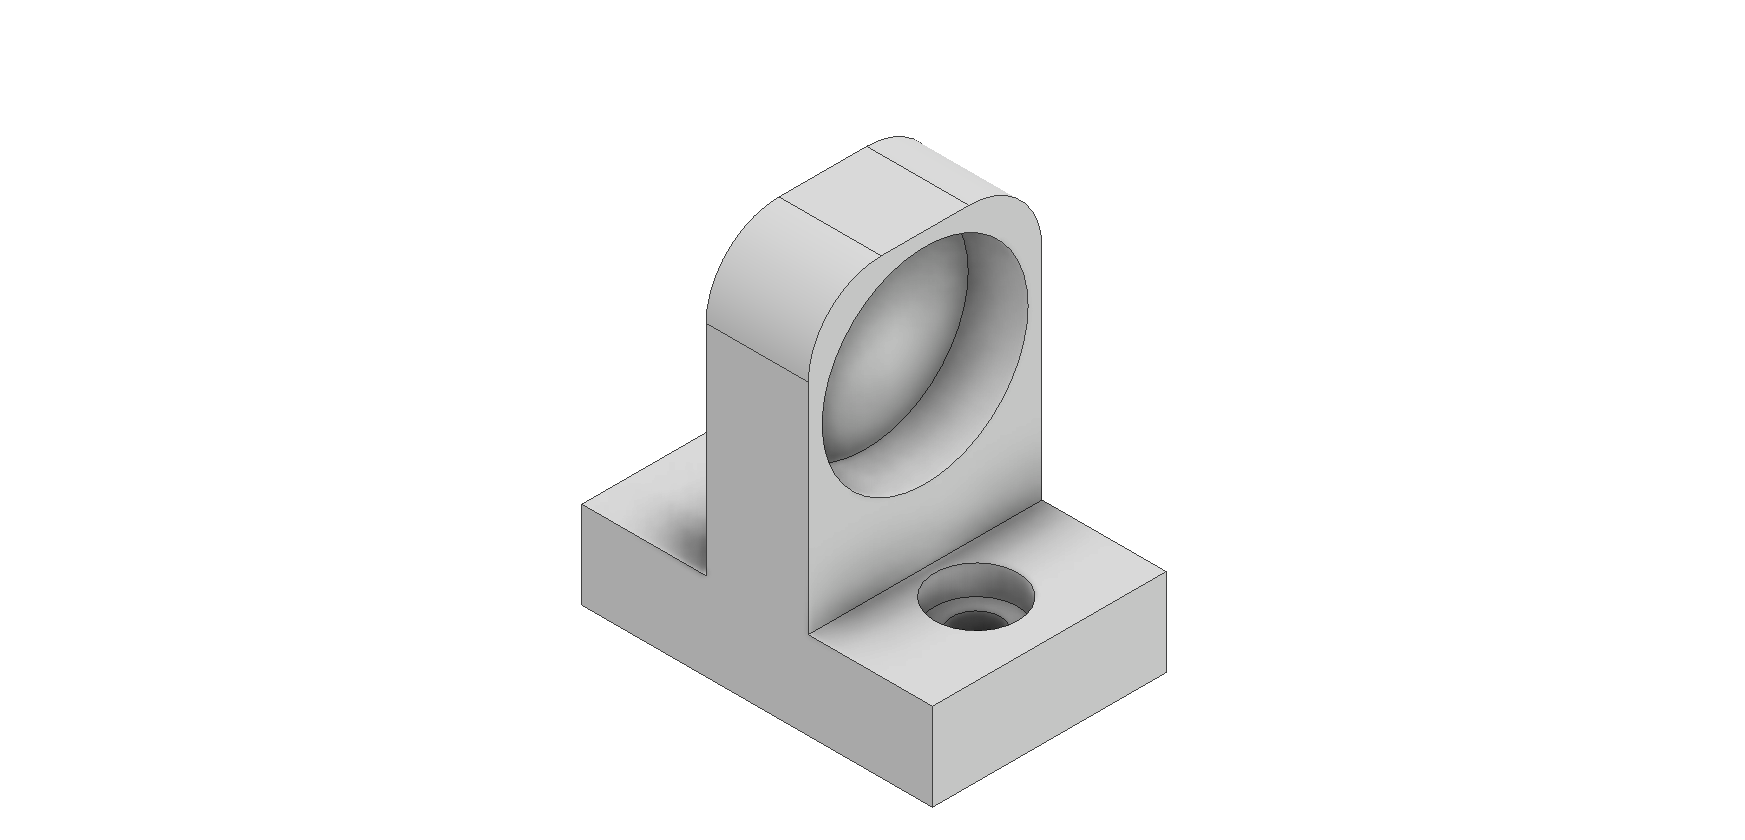
\includegraphics[width=\textwidth]{figures/ch3/fig3_22_b_Y_Bearing_Mount.png}
        \par (b) Y 軸軸承座
    \end{minipage}
    \vspace{0.5cm}
    \begin{minipage}[b]{0.48\textwidth}
        \centering
        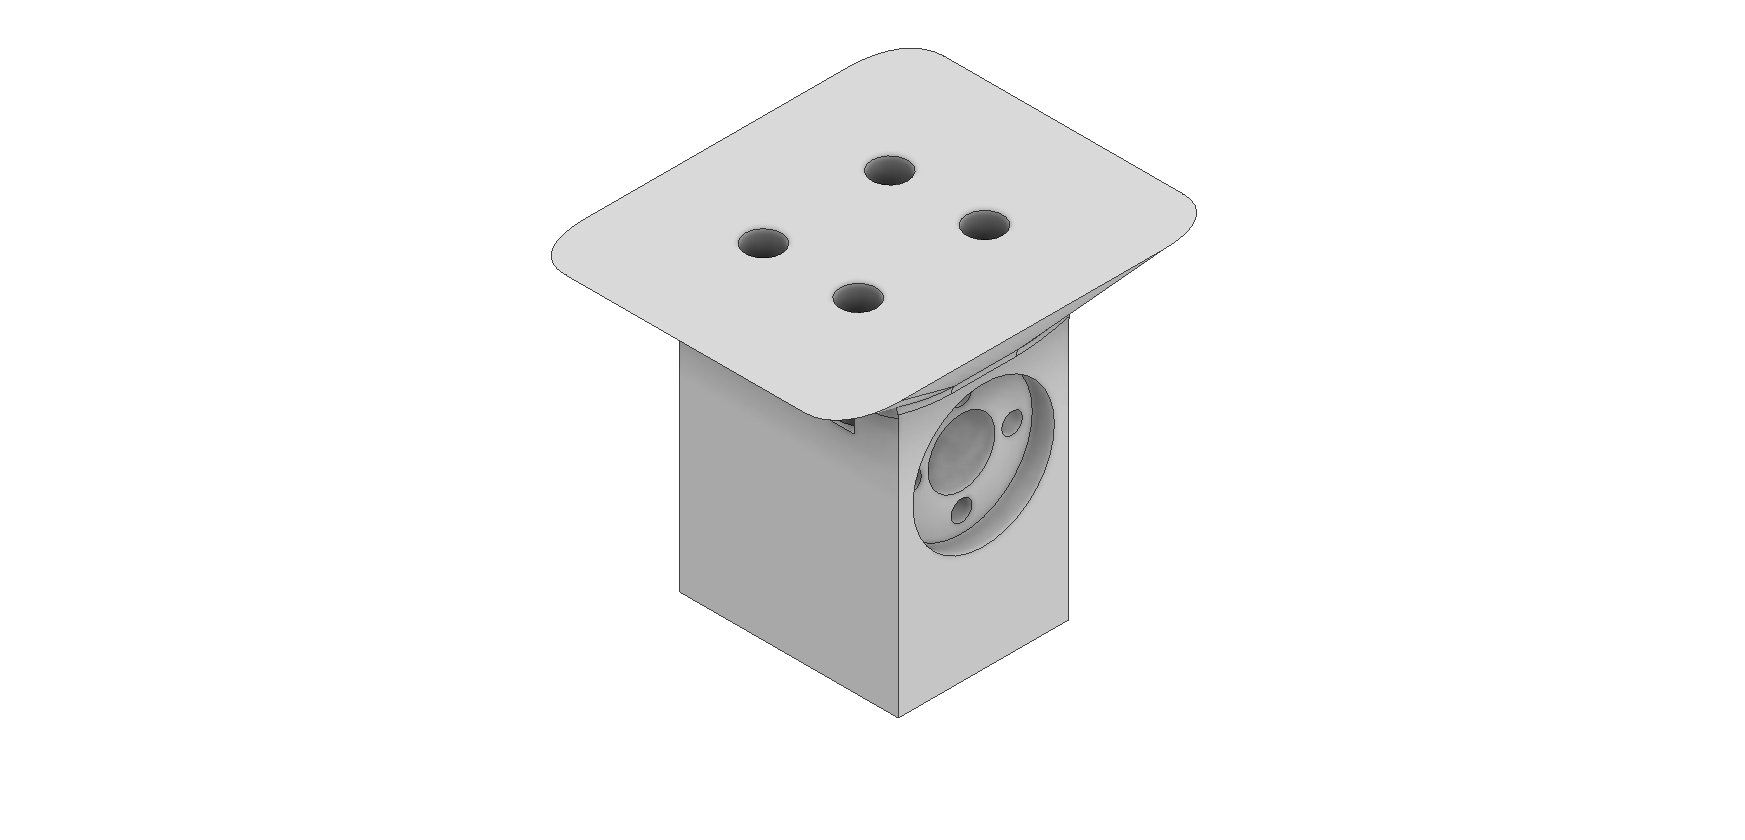
\includegraphics[width=\textwidth]{figures/ch3/fig3_22_c_Y_T8_Nut_Bracket.png}
        \par (c) Y 軸 T8 螺帽支架
    \end{minipage}
    \hfill
    \begin{minipage}[b]{0.48\textwidth}
        \centering
        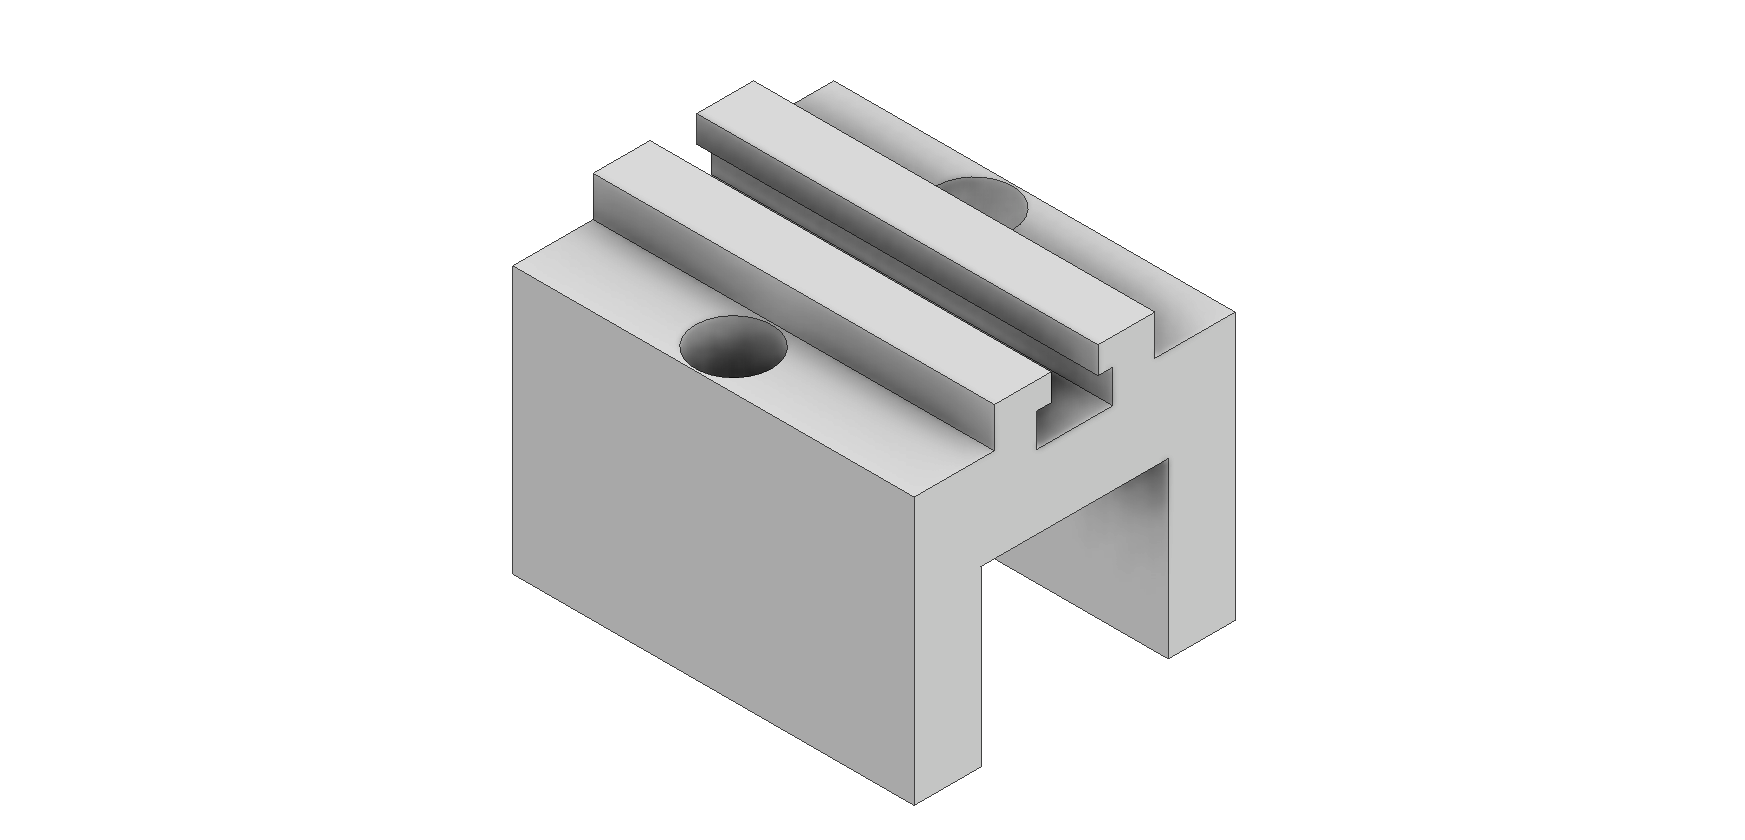
\includegraphics[width=\textwidth]{figures/ch3/fig3_22_d_Y_Rail_To_Bearing_Adapter.png}
        \par (d) Y 軸導軌至軸承轉接件
    \end{minipage}
    \vspace{0.5cm}
    \begin{minipage}[b]{0.9\textwidth}
        \centering
        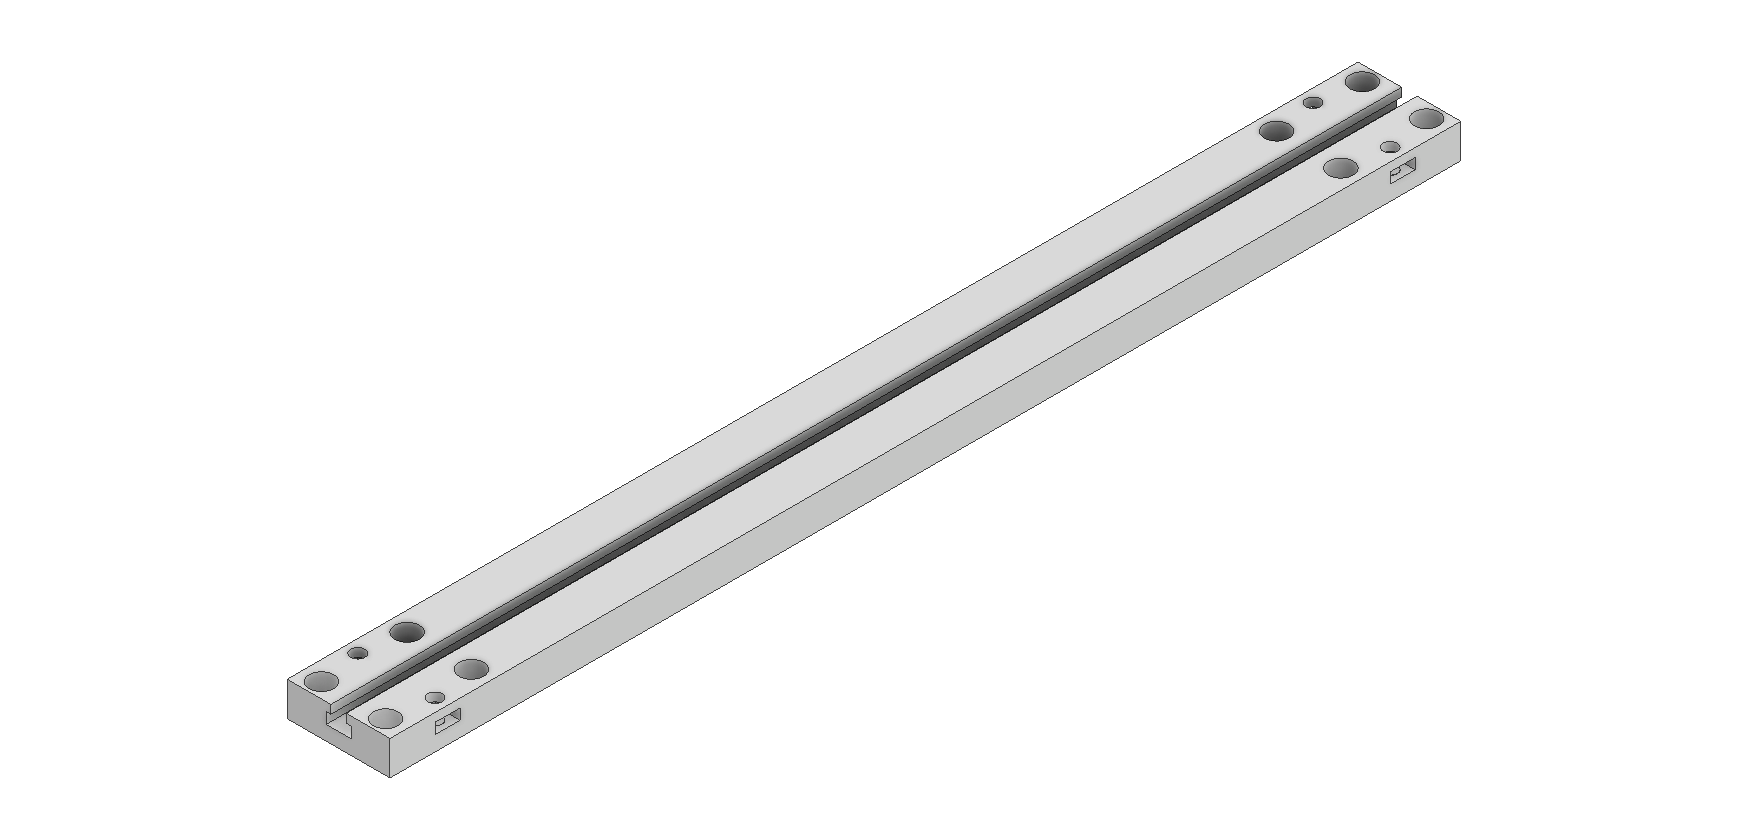
\includegraphics[width=\textwidth]{figures/ch3/fig3_22_e_Y_Rail_To_X_Adapter.png}
        \par (e) Y 軸至 X 軸轉接件
    \end{minipage}
    \caption{Y 軸部件}
    \label{fig:stage_y}
\end{figure}

Z 軸基座 (Z\_Axis\_Base)：構成 Z 軸（垂直對焦軸）的基礎剛性支架。此部件需要承受整個載台與樣本的垂直重力，為垂直運動提供了穩固的「地基」。

Z 軸螺帽支架 (Z\_Nut\_Bracket)：用於固定 Z 軸 T8 螺帽的機構件。當 Z 軸馬達旋轉時，此部件會帶動整個 X-Y 載台進行精密的垂直升降。它是實現微米級自動對焦（Auto-Focusing）的核心動力傳遞件。在本研究中，此機構亦用於採集 Z-Stack 斷層掃描資料以評估自動對焦演算法之效能；未來工作可進一步結合軟體擴展，實現全自動的 Z 軸斷層掃描成像。

樣本夾 (Sample\_Holder)：安裝於 X-Y 載台的最頂層，專為穩固夾持標準顯微鏡載玻片（Slides）所設計。其表面具有精密的定位靠邊，能有效防止載台在高速步進掃描時，樣本因慣性而發生微小滑移。

樣本固定夾 (Sample\_Clip)：配合樣本夾使用的彈性壓夾。當進行高倍率或長時程動態採集時，此固定夾能從上方提供溫和且均勻的壓力，將樣本緊緊貼合於基準面上，從而極大程度地抑制了環境震動帶來的離焦影響。

\begin{figure}[H]
    \centering
    \begin{minipage}[b]{0.48\textwidth}
        \centering
        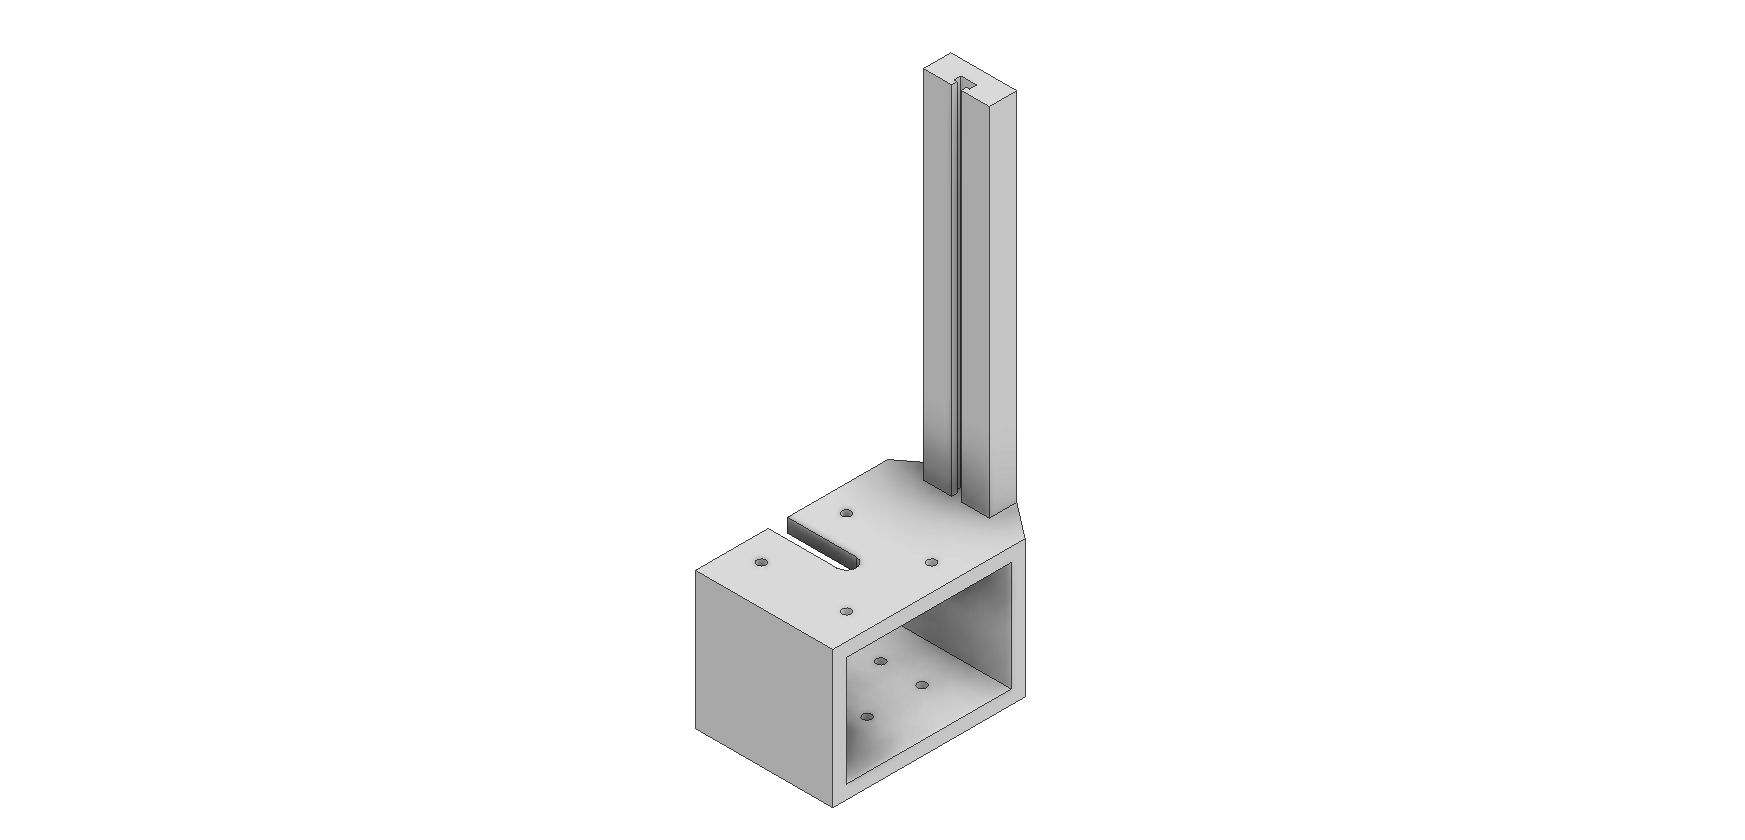
\includegraphics[width=\textwidth]{figures/ch3/fig3_23_a_Z_Axis_Base.png}
        \par (a) Z 軸基座
    \end{minipage}
    \hfill
    \begin{minipage}[b]{0.48\textwidth}
        \centering
        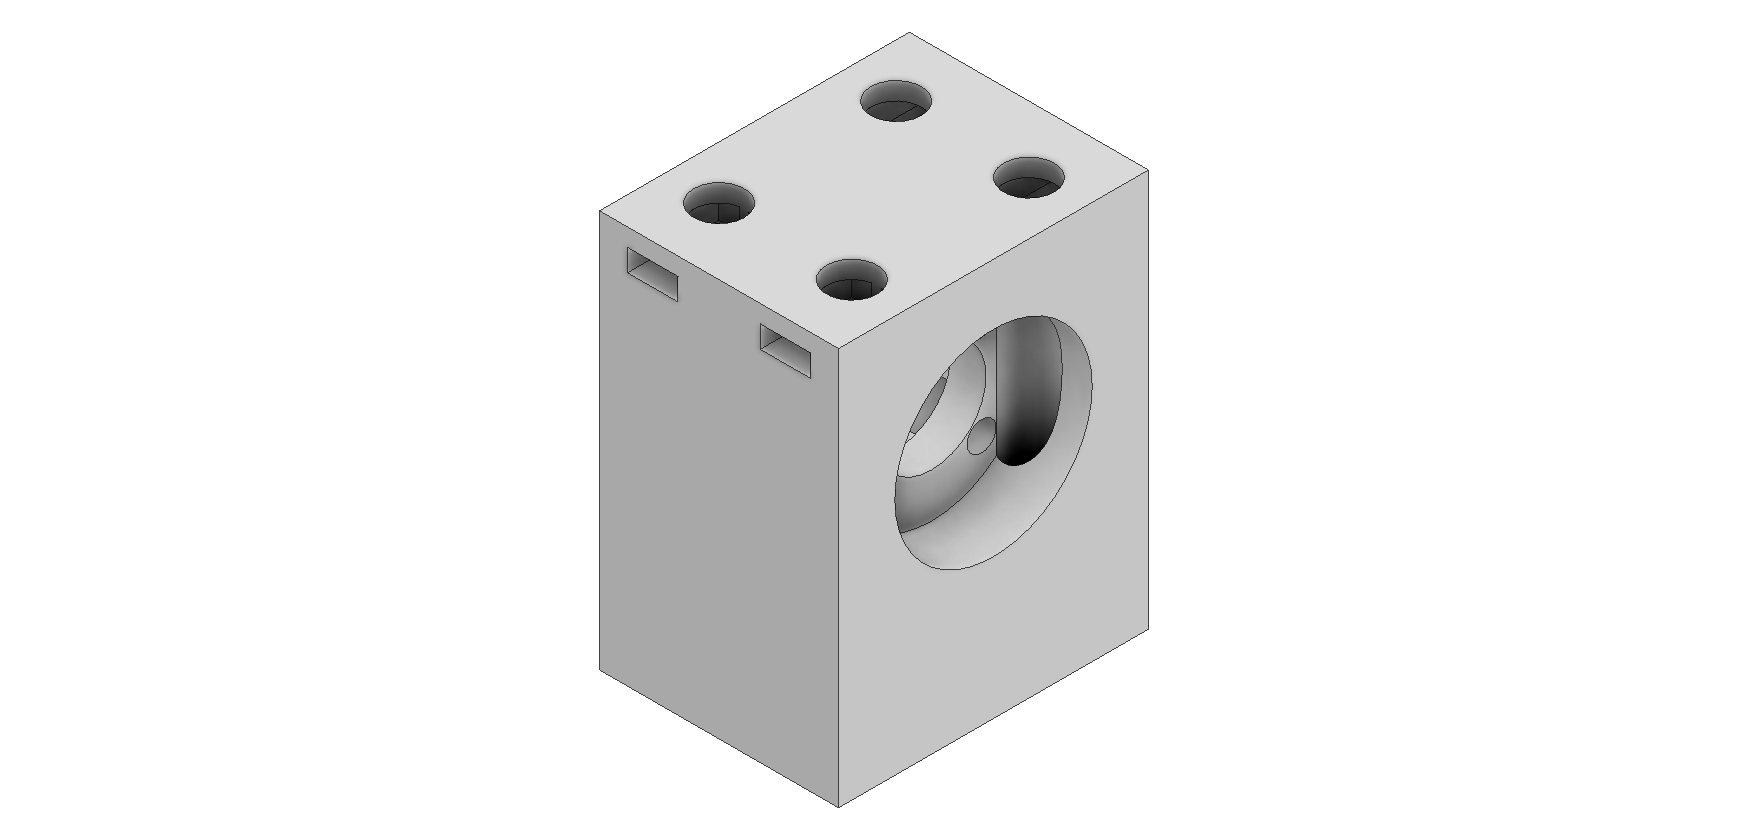
\includegraphics[width=\textwidth]{figures/ch3/fig3_23_b_Z_Nut_Bracket.png}
        \par (b) Z 軸螺帽支架
    \end{minipage}
    \vspace{0.5cm}
    \begin{minipage}[b]{0.48\textwidth}
        \centering
        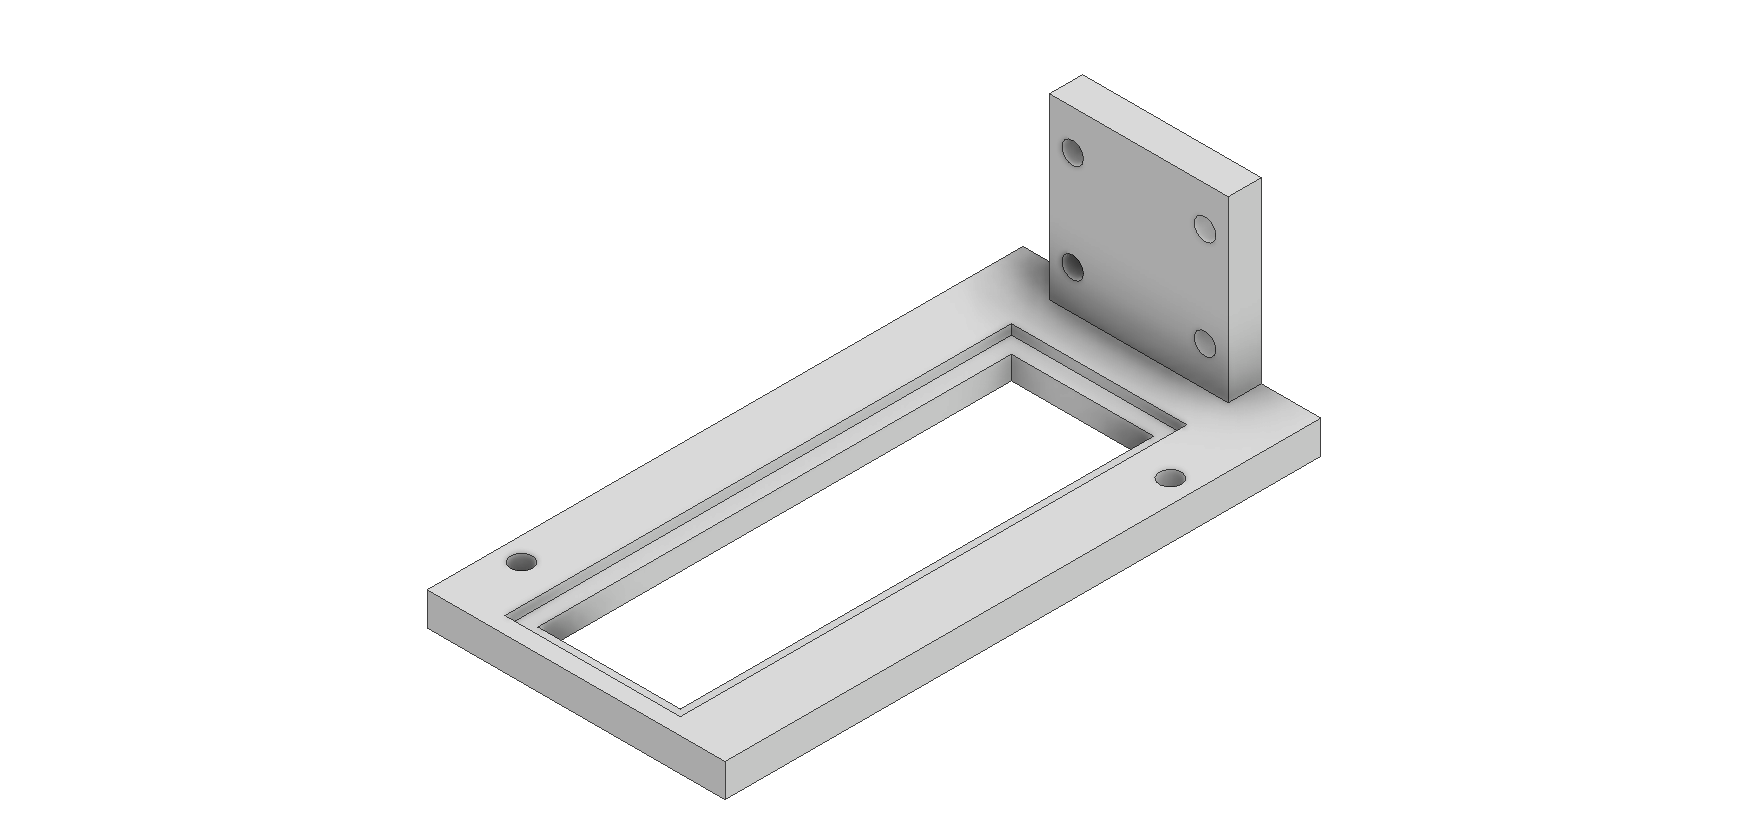
\includegraphics[width=\textwidth]{figures/ch3/fig3_23_c_Sample_Holder.png}
        \par (c) 樣本夾
    \end{minipage}
    \hfill
    \begin{minipage}[b]{0.48\textwidth}
        \centering
        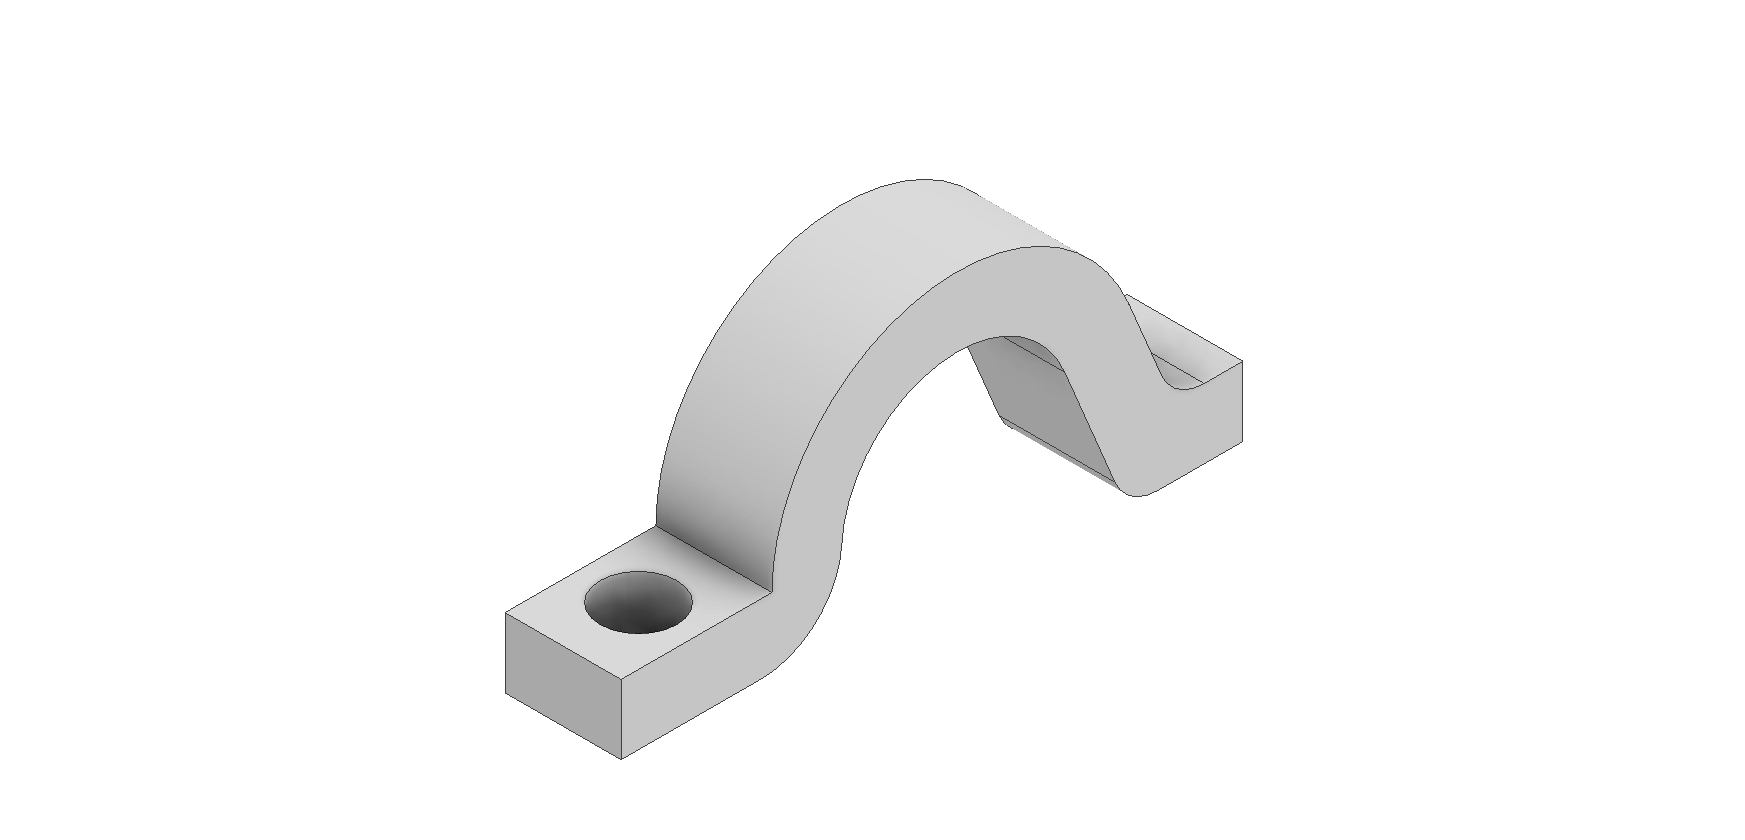
\includegraphics[width=\textwidth]{figures/ch3/fig3_23_d_Sample_Clip.png}
        \par (d) 樣本固定夾
    \end{minipage}
    \caption{Z 軸與樣本夾部件}
    \label{fig:stage_z}
\end{figure}


為了進一步提升實驗操作的便利性，我們在濾光方塊等光學固定座上引入了人性化的「鑷子夾取槽」設計，讓使用者在不必拆卸周邊元件的情況下，即可用鑷子夾取光學元件並快速更換。同時，濾光方塊與激發濾光片座採用「推到底即定位」的防呆設計，確保每次更換後均能放入合適的位置（如圖 \ref{fig:design_tweezers_and_push} 所示）。

\begin{figure}[H]
    \centering
    \begin{minipage}[b]{0.8\textwidth}
        \centering
        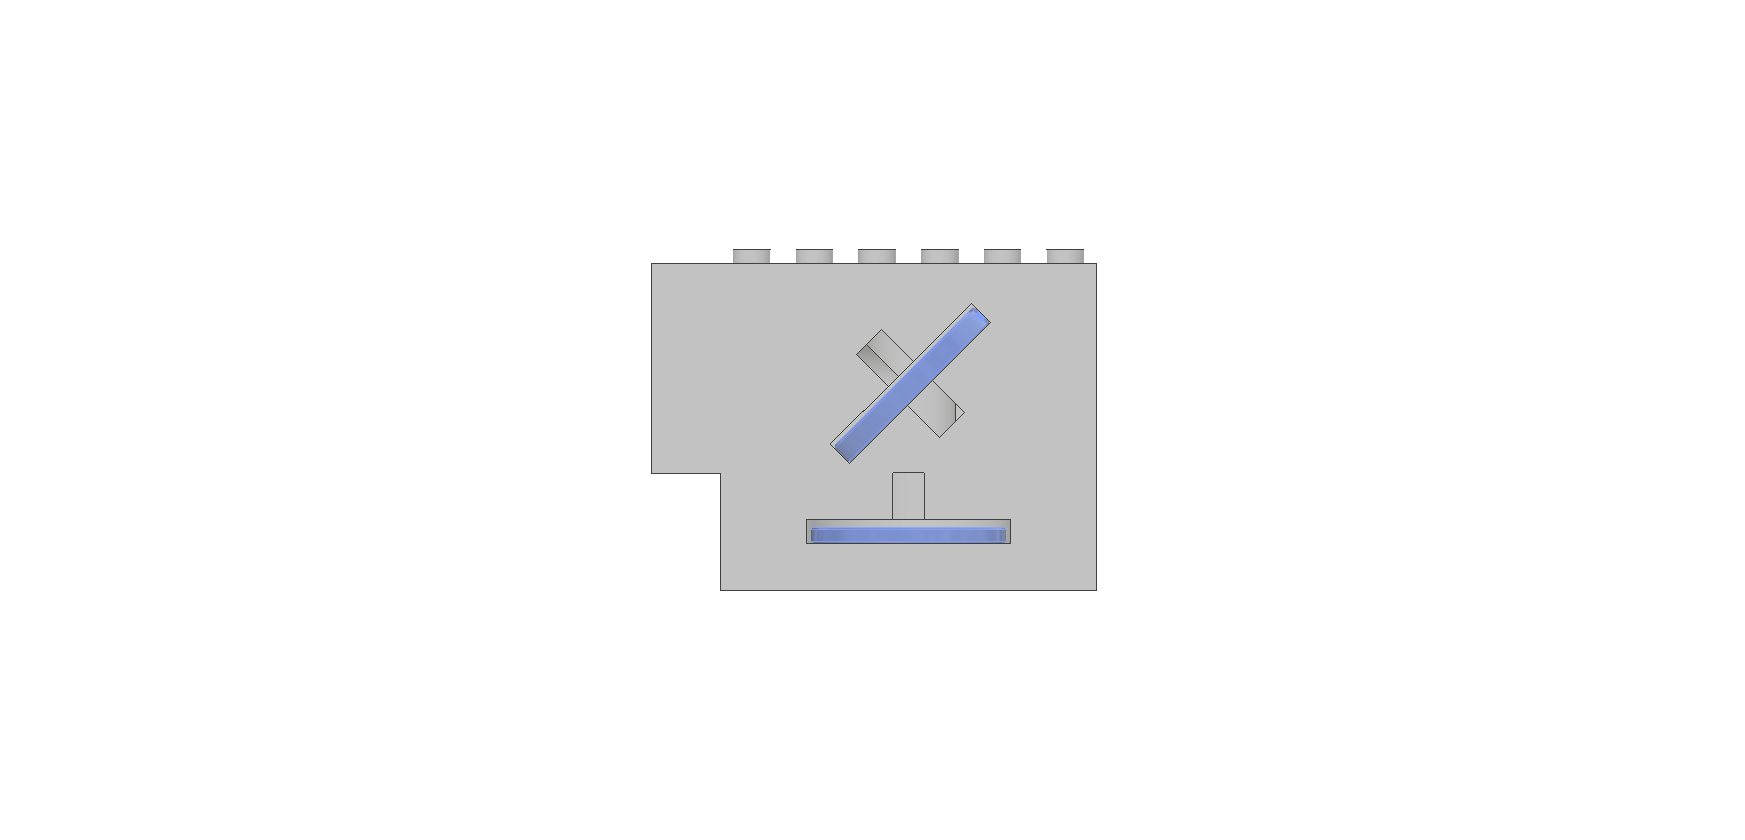
\includegraphics[width=\textwidth]{figures/ch3/fig3_24_a_Filter_Cube_Tweezers_Slot.png}
        \par (a) 濾光方塊鑷子夾取槽
    \end{minipage}
    \vspace{0.5cm}
    
    \begin{minipage}[b]{0.48\textwidth}
        \centering
        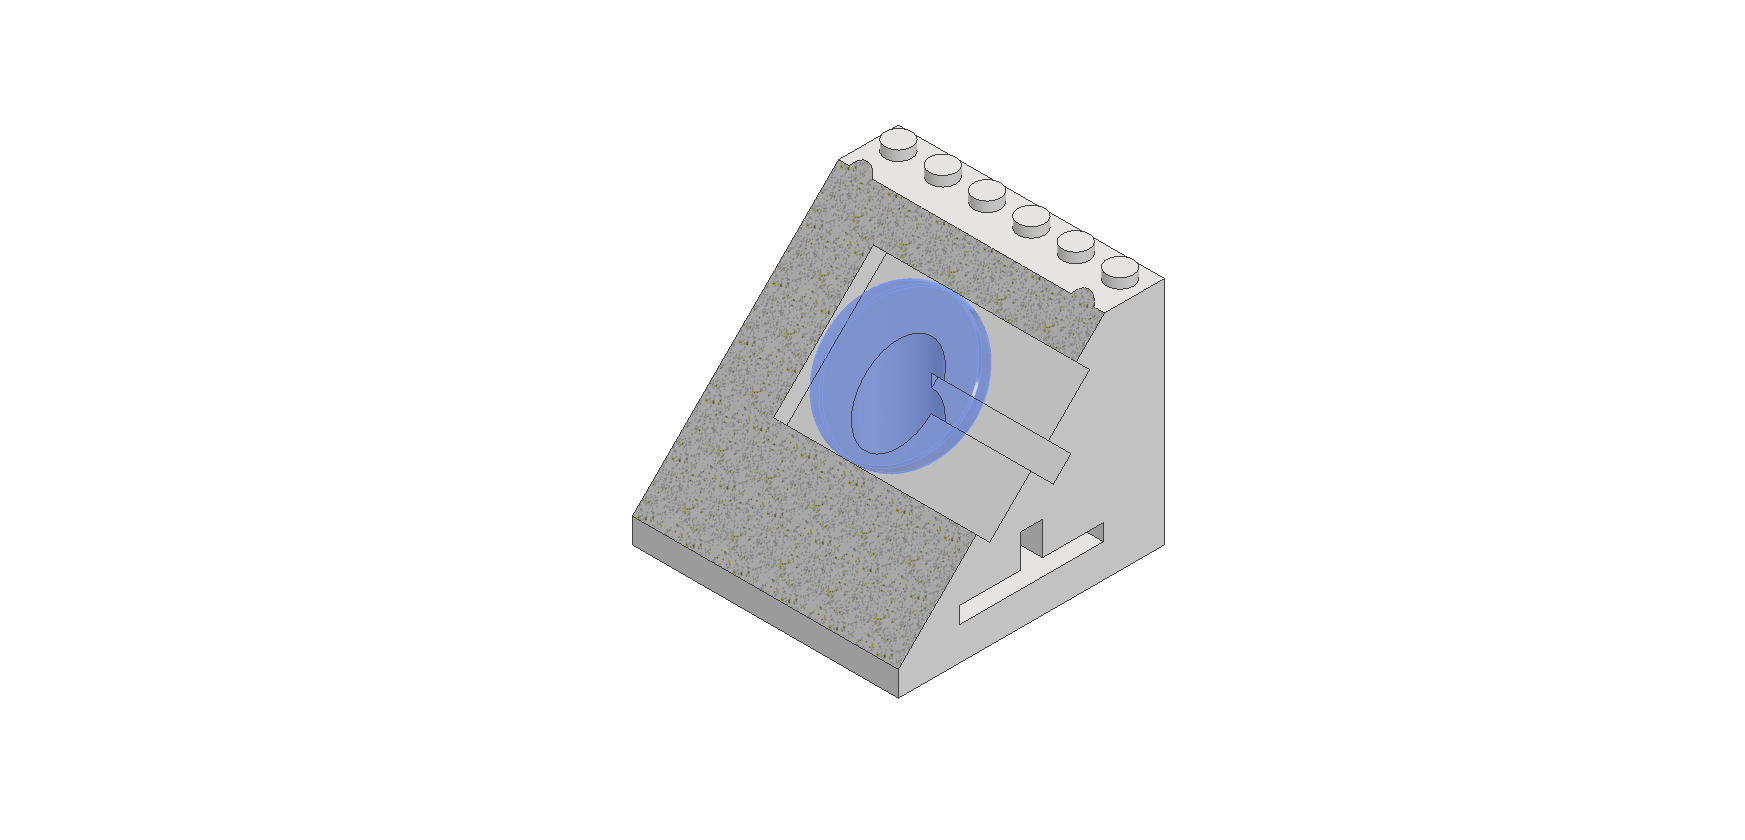
\includegraphics[width=\textwidth]{figures/ch3/fig3_24_b_DM_Push_To_Locate.png}
        \par (b) 分光鏡推到底設計
    \end{minipage}
    \hfill
    \begin{minipage}[b]{0.48\textwidth}
        \centering
        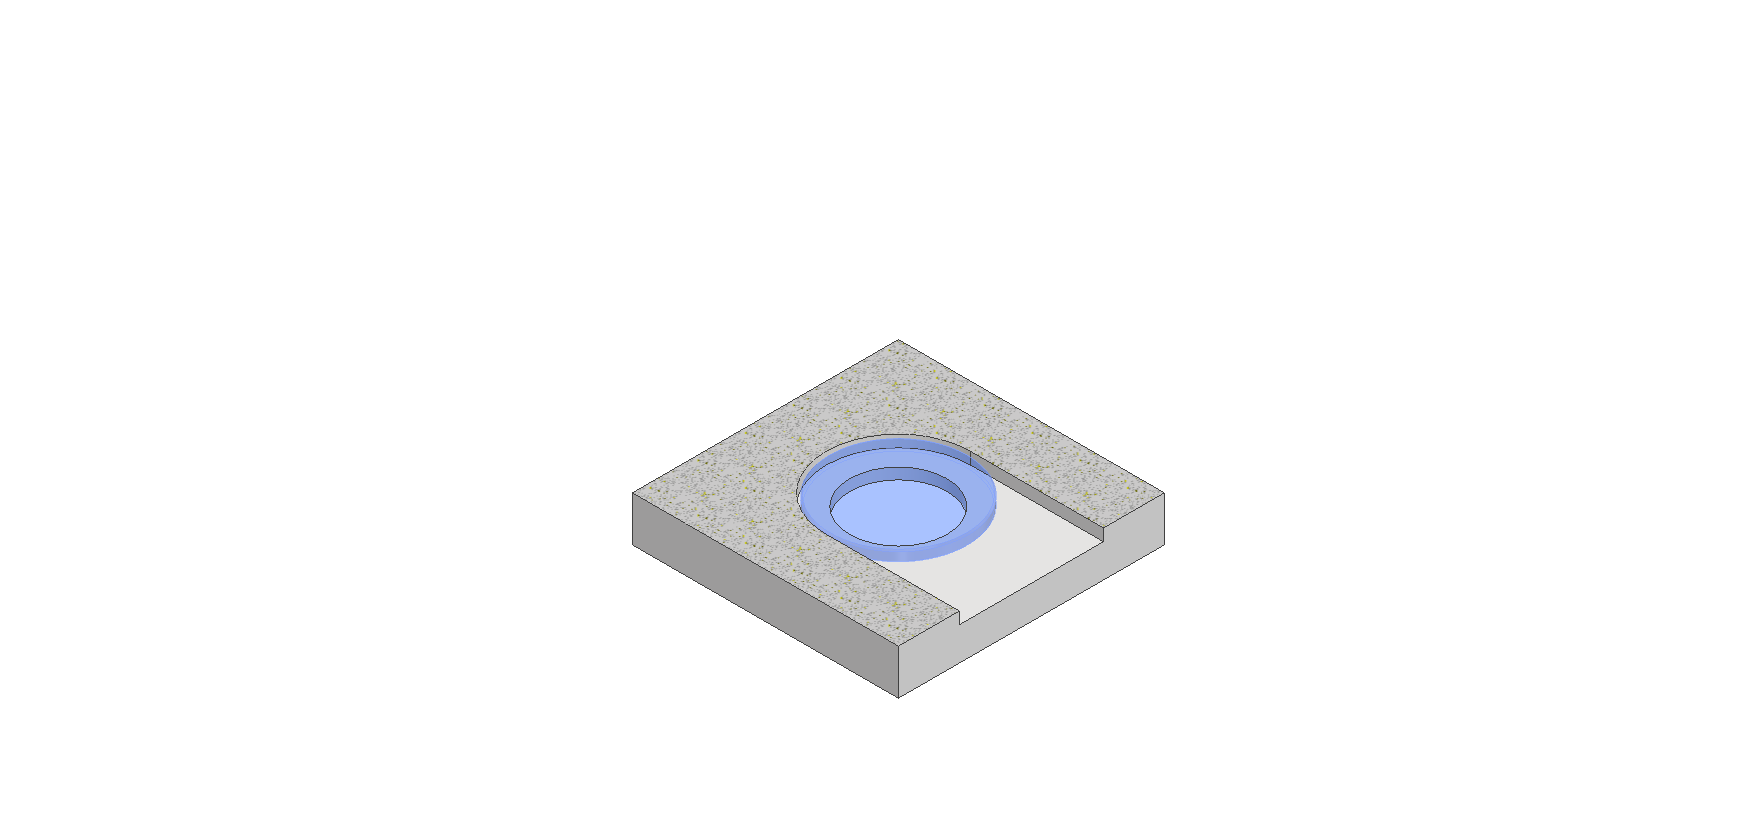
\includegraphics[width=\textwidth]{figures/ch3/fig3_24_c_Ex_Filter_Push_To_Locate.png}
        \par (c) 激發片推到底設計
    \end{minipage}
    \caption{濾光方塊與濾光片之抽換與定位設計}
    \label{fig:design_tweezers_and_push}
\end{figure}

此外，在 \texttt{Diffuser\_Mount}（擴散片座）上，除了設有鑷子夾取槽外，內部亦設計有圓弧導引槽，利用重力原理使濾光片放入後能自動擺正至最佳位置（如圖 \ref{fig:design_diffuser} 所示）。

\begin{figure}[H]
    \centering
    \begin{minipage}[b]{0.48\textwidth}
        \centering
        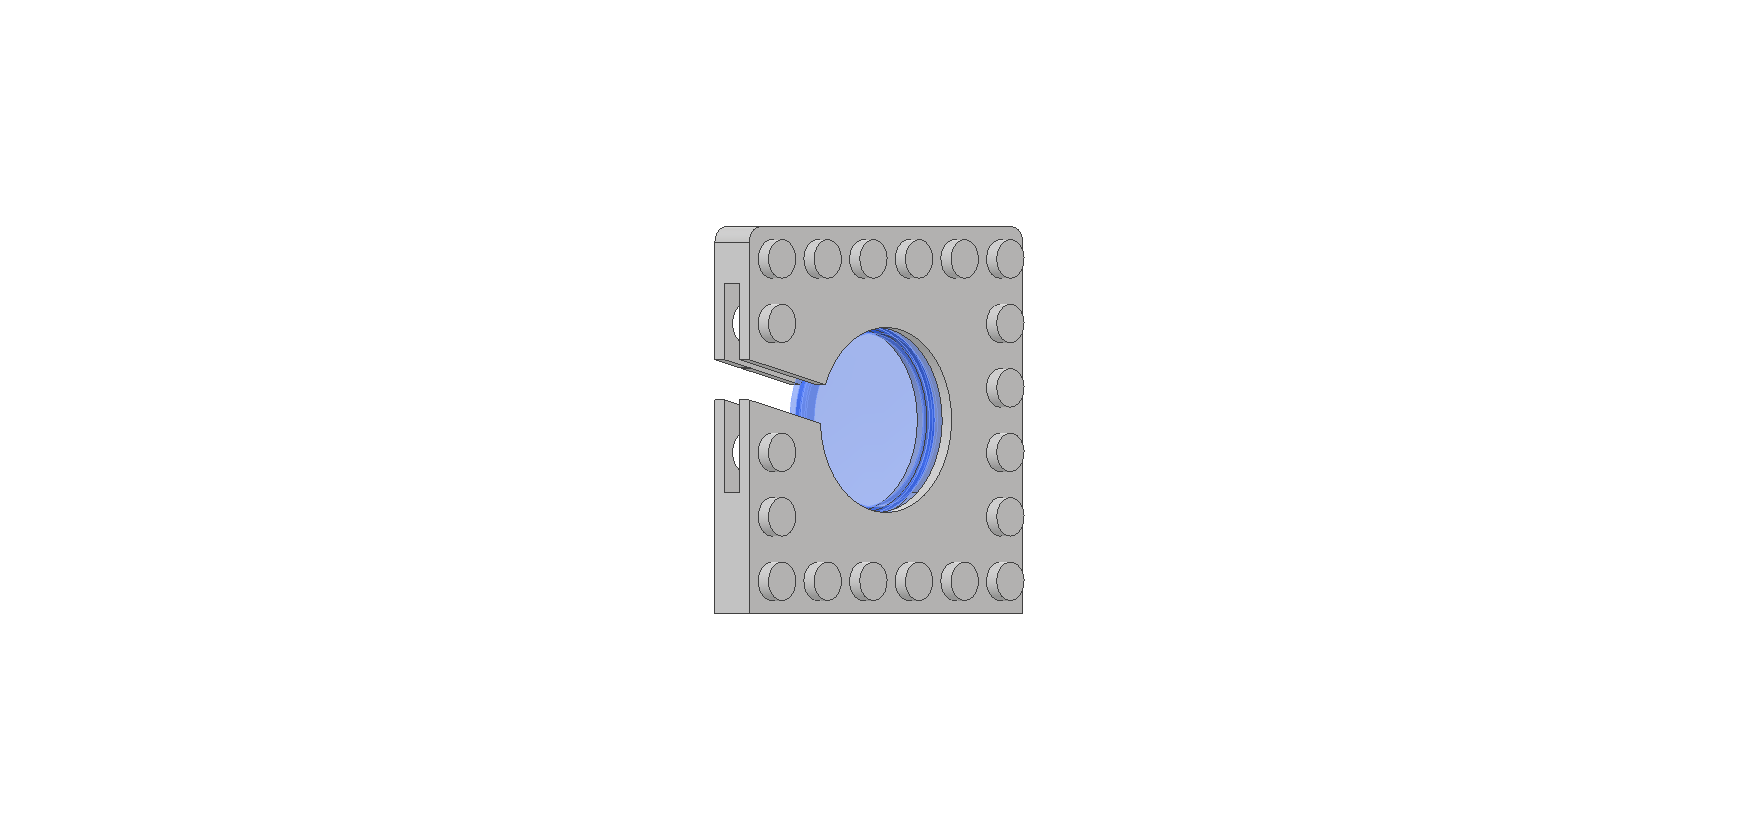
\includegraphics[width=\textwidth]{figures/ch3/fig3_25_a_Diffuser_Mount_Tweezers_Slot.png}
        \par (a) 鑷子夾取槽設計
    \end{minipage}
    \hfill
    \begin{minipage}[b]{0.48\textwidth}
        \centering
        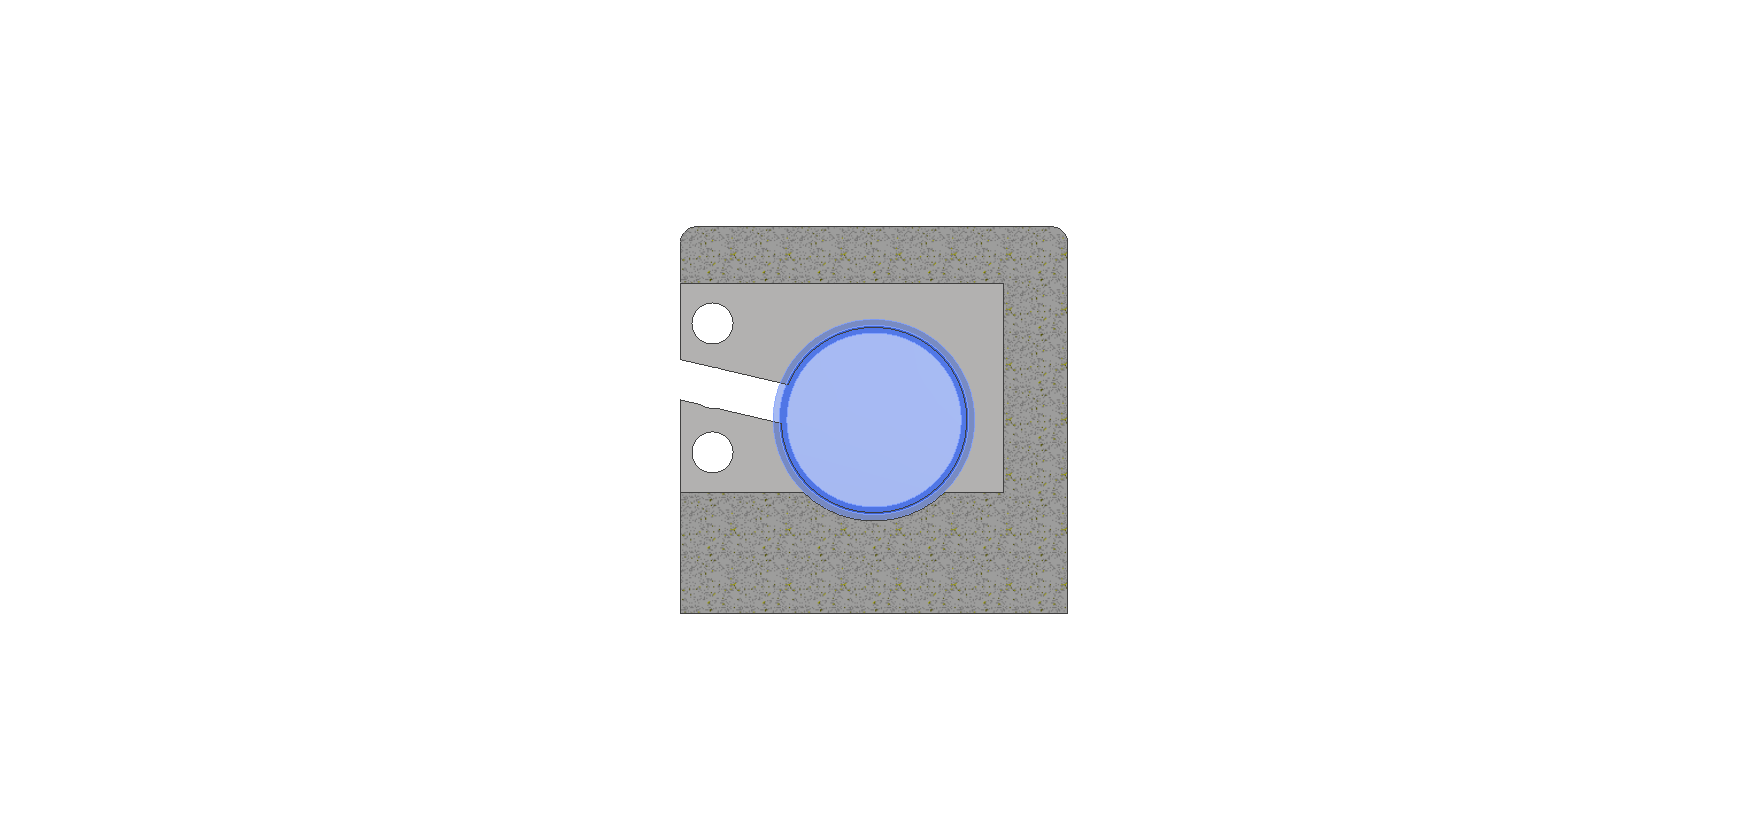
\includegraphics[width=\textwidth]{figures/ch3/fig3_25_b_Diffuser_Self_Aligning_Arc.png}
        \par (b) 圓弧自擺正設計
    \end{minipage}
    \caption{擴散片座之細節設計}
    \label{fig:design_diffuser}
\end{figure}

同樣地，在 \texttt{Excitation\_Filter\_Mount}（激發濾光片座）上，也集成了鑷子夾取槽、圓弧自擺正以及與濾光方塊連接的卡榫結構，以提升更換濾光片時的便利性與精準度（如圖 \ref{fig:design_excitation} 所示）。

\begin{figure}[H]
    \centering
    \begin{minipage}[b]{0.48\textwidth}
        \centering
        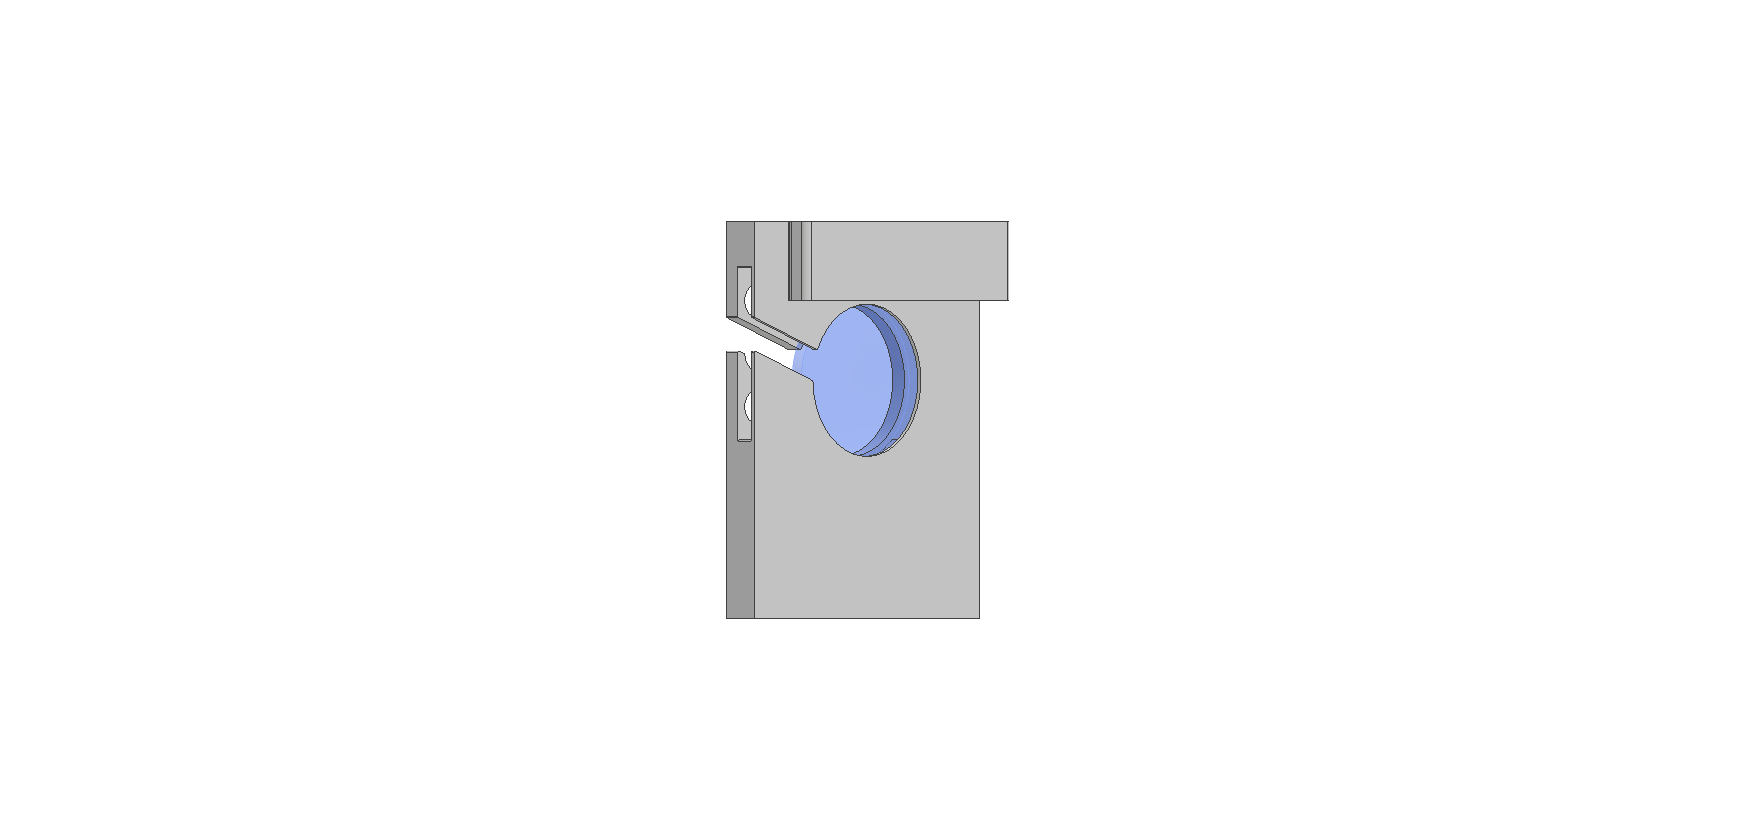
\includegraphics[width=\textwidth]{figures/ch3/fig3_26_a_Excitation_Mount_Tweezers_Slot.png}
        \par (a) 鑷子夾取槽設計
    \end{minipage}
    \hfill
    \begin{minipage}[b]{0.48\textwidth}
        \centering
        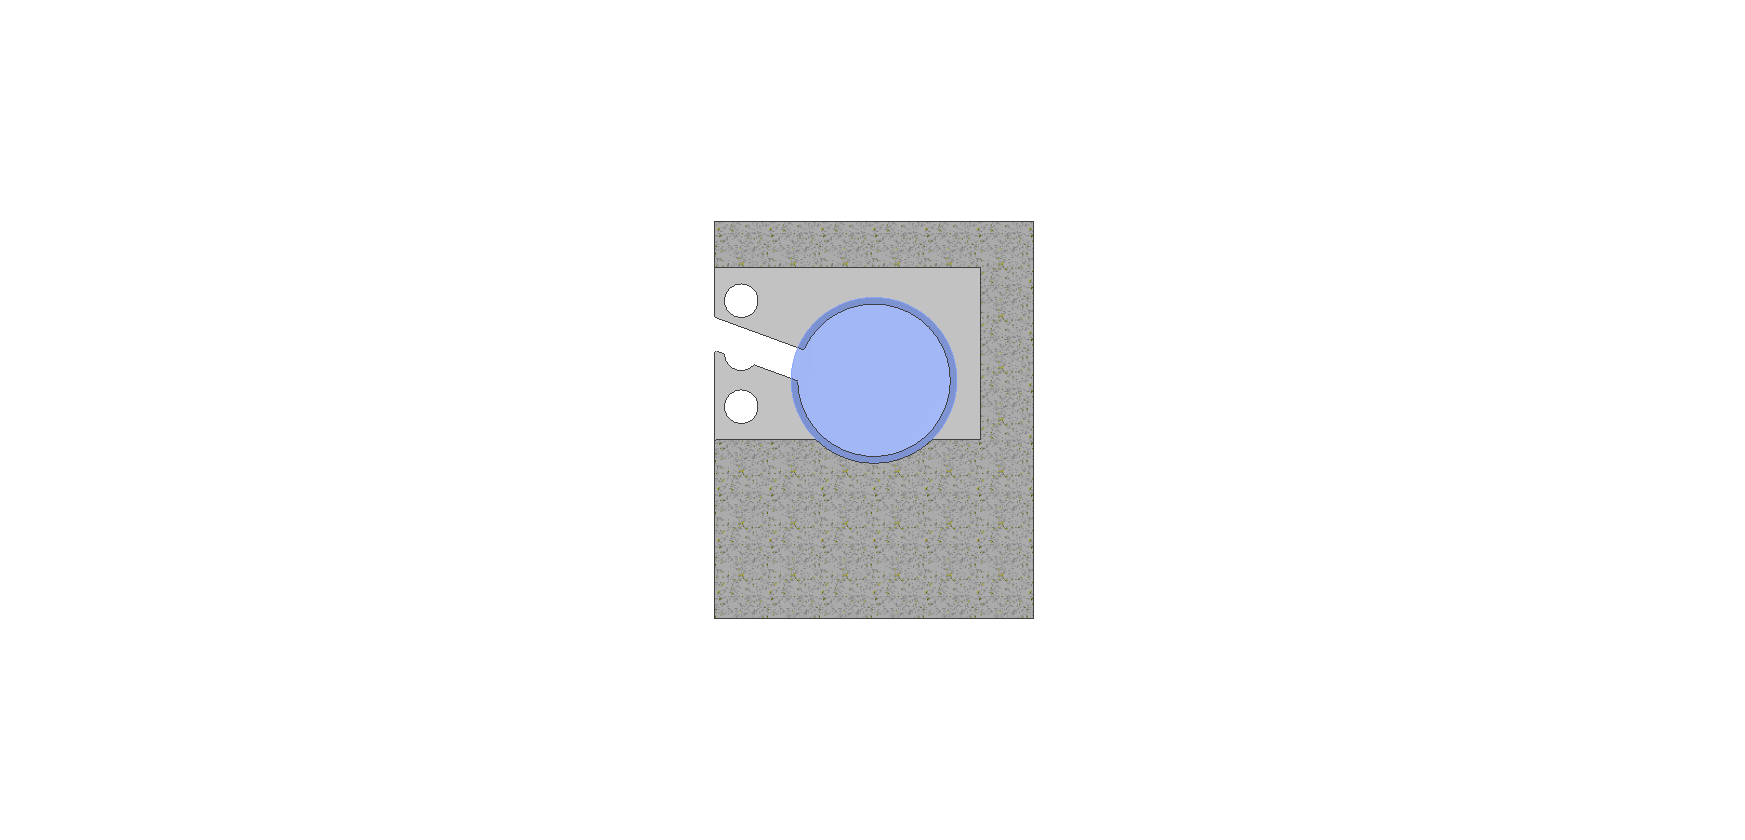
\includegraphics[width=\textwidth]{figures/ch3/fig3_26_b_Excitation_Self_Aligning_Arc.png}
        \par (b) 圓弧自擺正設計
    \end{minipage}
    \caption{激發濾光片座之細節設計}
    \label{fig:design_excitation}
\end{figure}

此外，本系統在結構設計上也融入了多項對齊與支撐的巧思。除了利用樂高積木的標準孔距進行大部對齊外，我們在濾光方塊與激發濾光片座等關鍵對齊部件上，設計了微型的「卡榫（Mortise and Tenon）」結構，確保其次微米級的對齊精度（如圖 \ref{fig:design_alignment} 所示）。而在聚光鏡的安裝上，為了確保光學元件的同軸度與穩定性，我們採用了類似「內縮三角形」的概念，透過三點約束（Three-Point Constraint）的方式將聚光鏡牢固地支撐住，有效避免了傳統圓形套筒可能產生的偏擺（如圖 \ref{fig:design_3point_bf} 與圖 \ref{fig:design_3point_fluo} 所示）。

\begin{figure}[H]
    \centering
    \begin{minipage}[b]{0.48\textwidth}
        \centering
        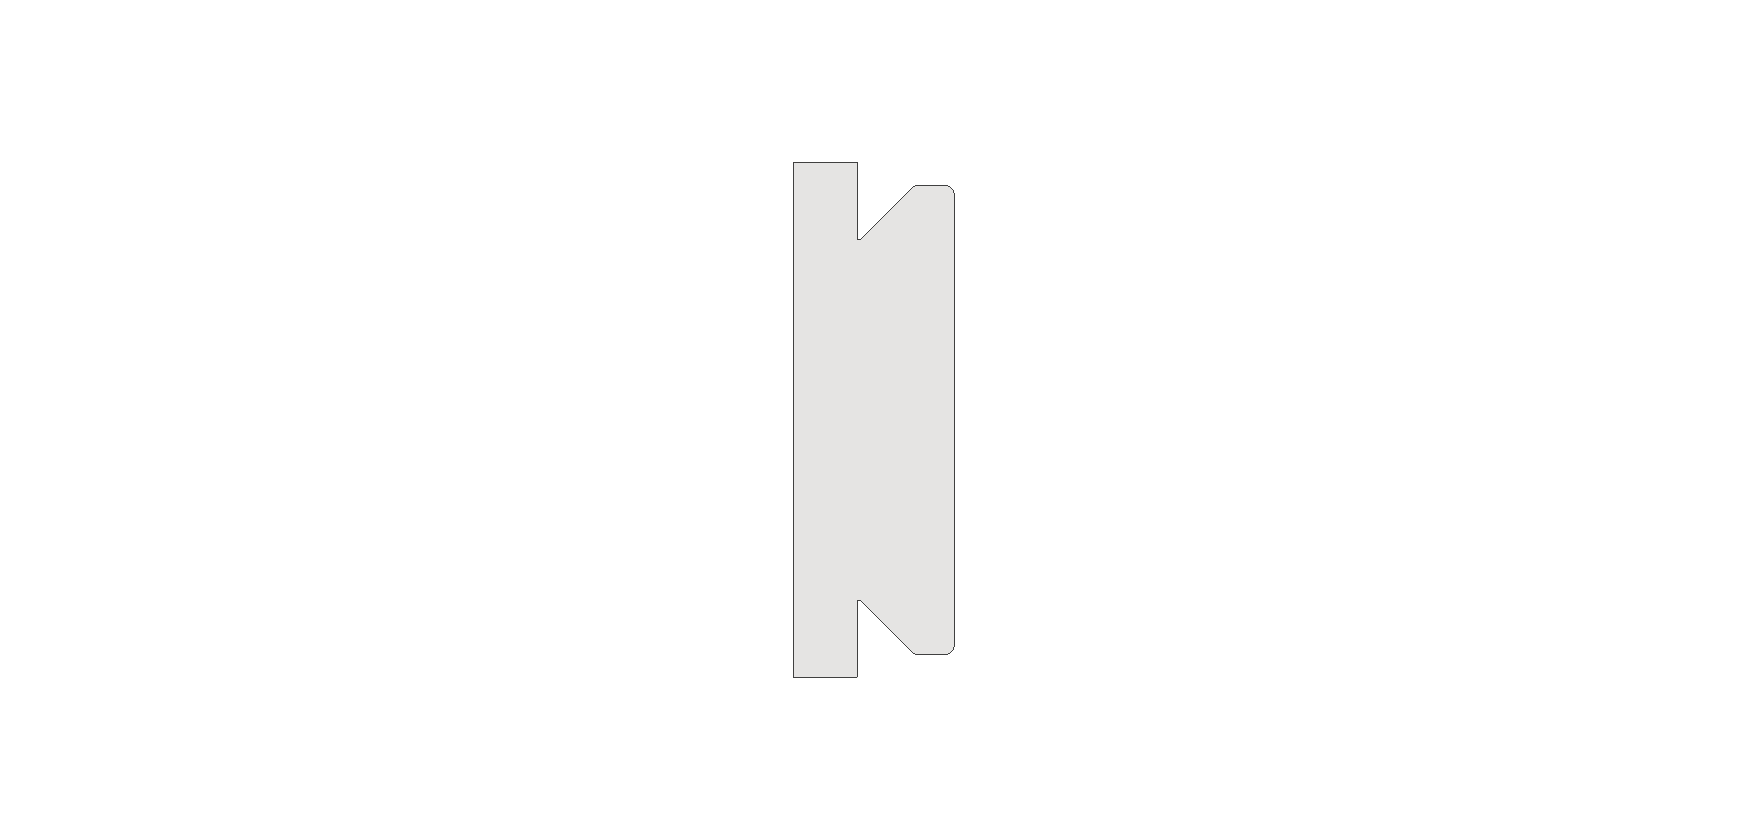
\includegraphics[width=\textwidth]{figures/ch3/fig3_27_a_Ex_Filter_Mortise_Tenon.png}
        \par (a) 激發濾光片座卡榫
    \end{minipage}
    \hfill
    \begin{minipage}[b]{0.48\textwidth}
        \centering
        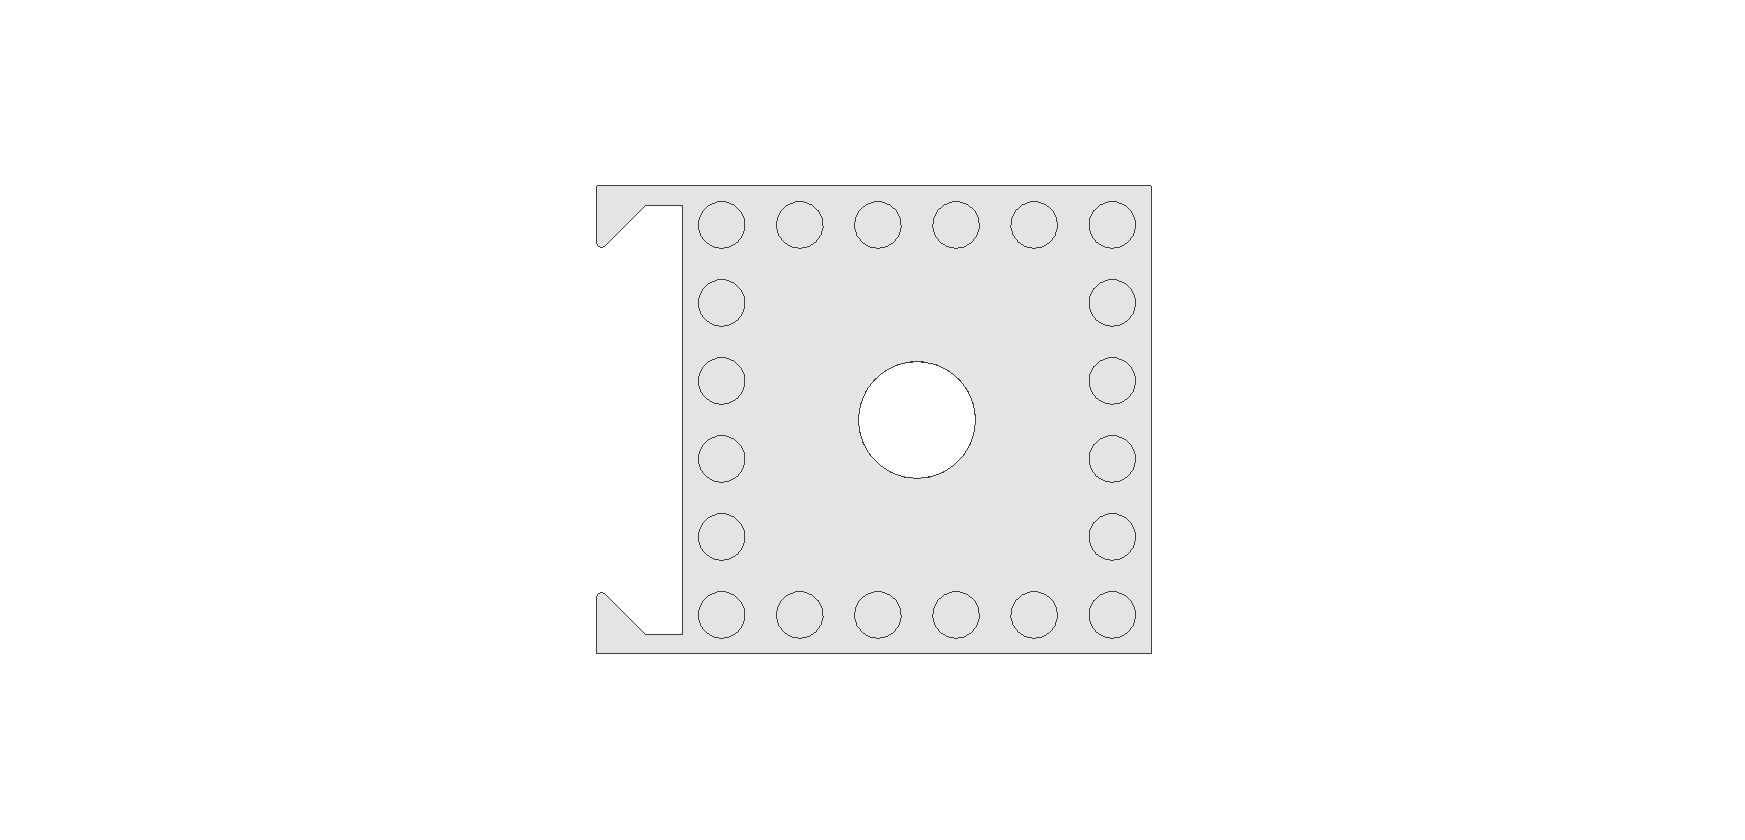
\includegraphics[width=\textwidth]{figures/ch3/fig3_27_b_Filter_Cube_Mortise_Tenon.png}
        \par (b) 濾光方塊卡榫結構
    \end{minipage}
    \vspace{0.5cm}
    
    \begin{minipage}[b]{0.8\textwidth}
        \centering
        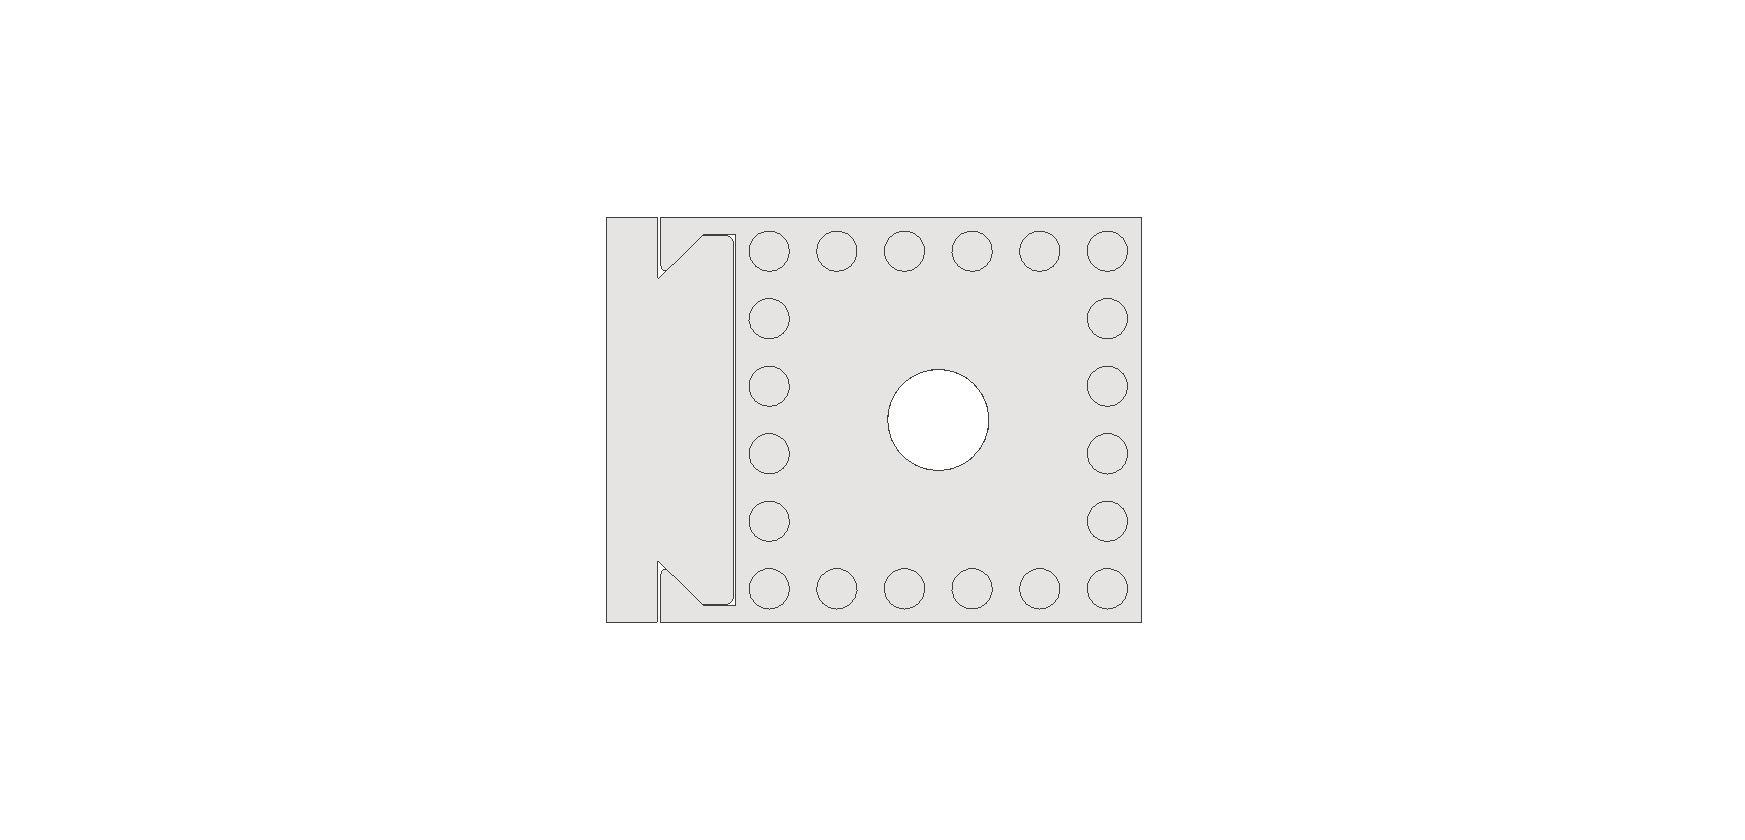
\includegraphics[width=\textwidth]{figures/ch3/fig3_27_c_Cube_Ex_Filter_Mortise_Tenon_Assembly.png}
        \par (c) 卡榫整體對齊示意圖
    \end{minipage}
    \caption{濾光方塊與激發濾光片座之卡榫設計與對齊示意圖}
    \label{fig:design_alignment}
\end{figure}

\begin{figure}[H]
    \centering
    \begin{minipage}[b]{0.48\textwidth}
        \centering
        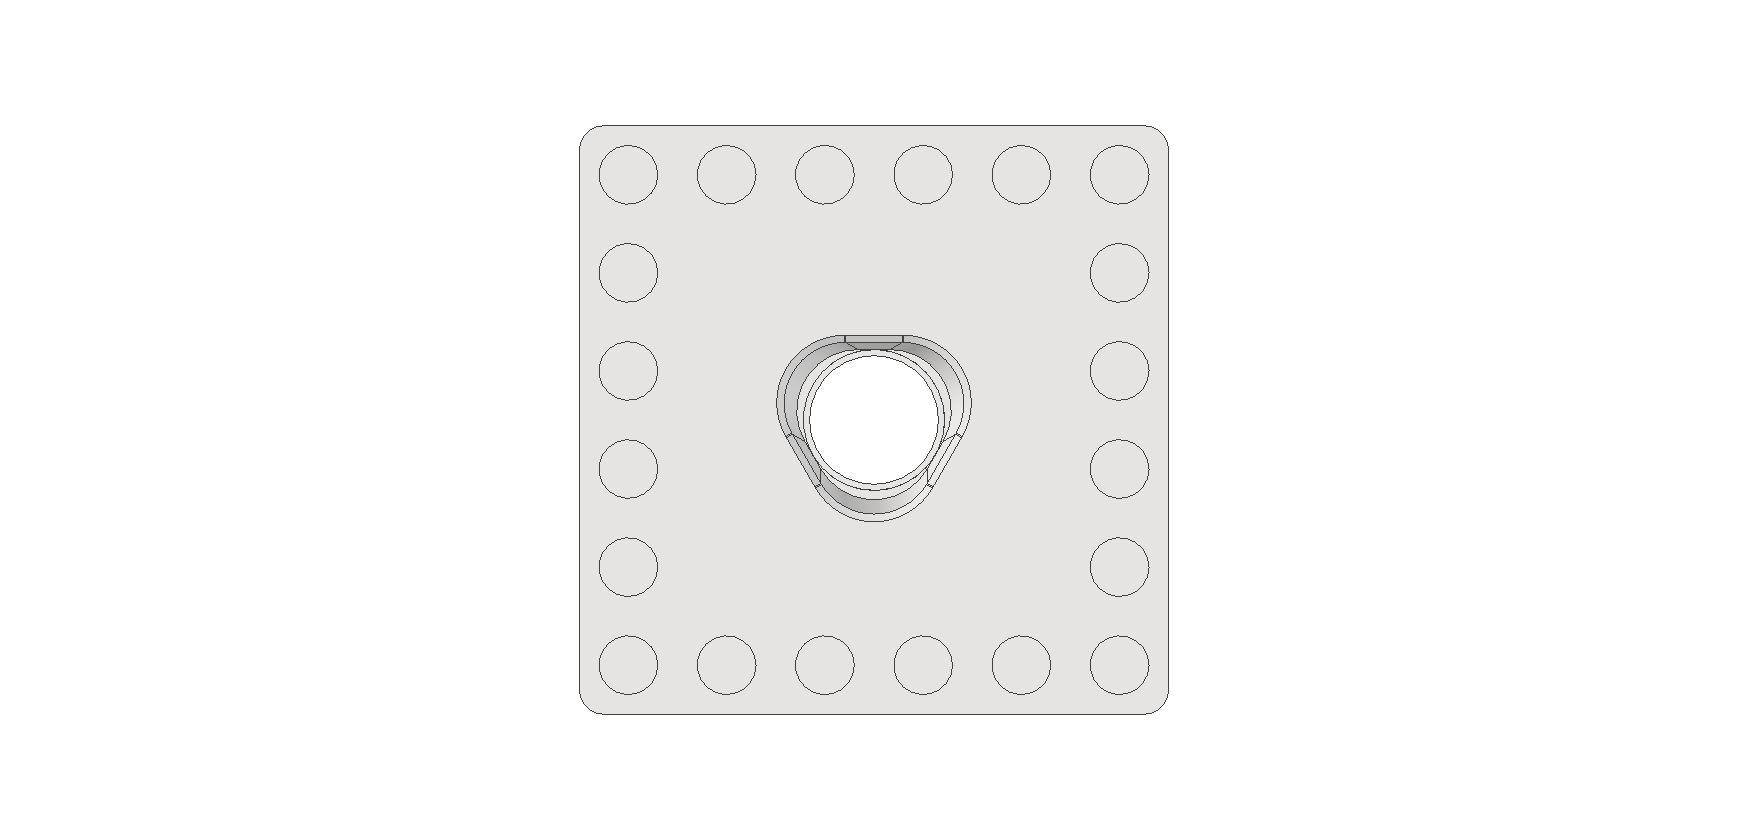
\includegraphics[width=\textwidth]{figures/ch3/fig3_28_a_BF_Condenser_Three_Point_Constraint.png}
        \par (a) 明視野聚光鏡 3點設計
    \end{minipage}
    \hfill
    \begin{minipage}[b]{0.48\textwidth}
        \centering
        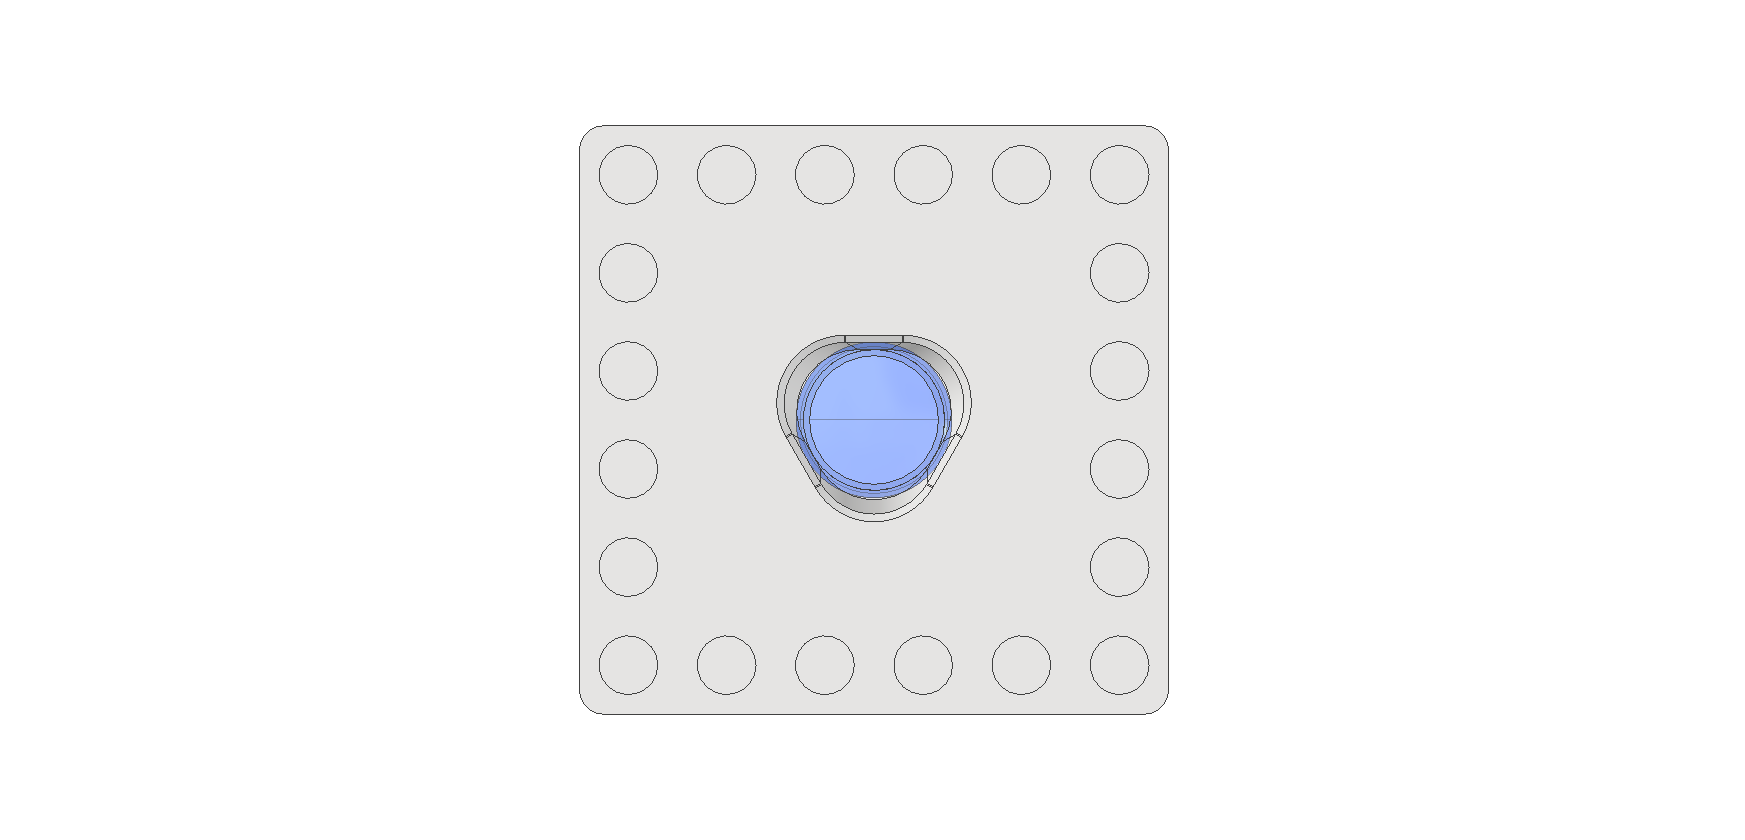
\includegraphics[width=\textwidth]{figures/ch3/fig3_28_b_BF_Condenser_Assembly.png}
        \par (b) 明視野聚光鏡組裝
    \end{minipage}
    \vspace{0.5cm}
    
    \begin{minipage}[b]{0.8\textwidth}
        \centering
        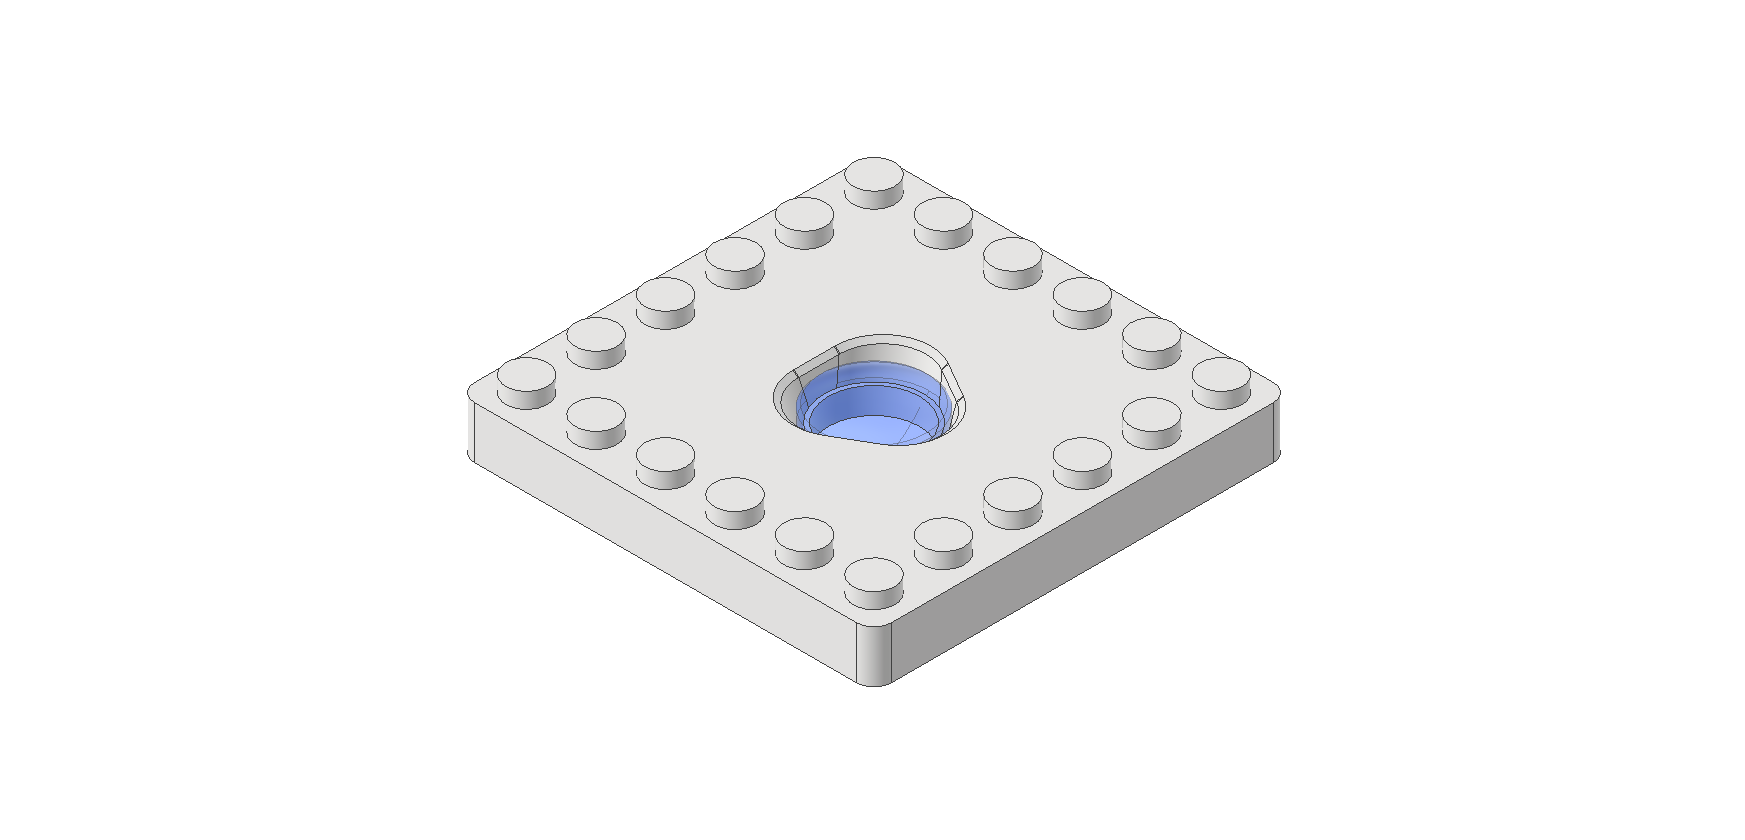
\includegraphics[width=\textwidth]{figures/ch3/fig3_28_c_BF_Condenser_Three_Point_3.png}
        \par (c) 45度視角的組裝
    \end{minipage}
    \caption{明視野聚光鏡之三點約束（Three-Point Constraint）支撐設計}
    \label{fig:design_3point_bf}
\end{figure}

\begin{figure}[H]
    \centering
    \begin{minipage}[b]{0.48\textwidth}
        \centering
        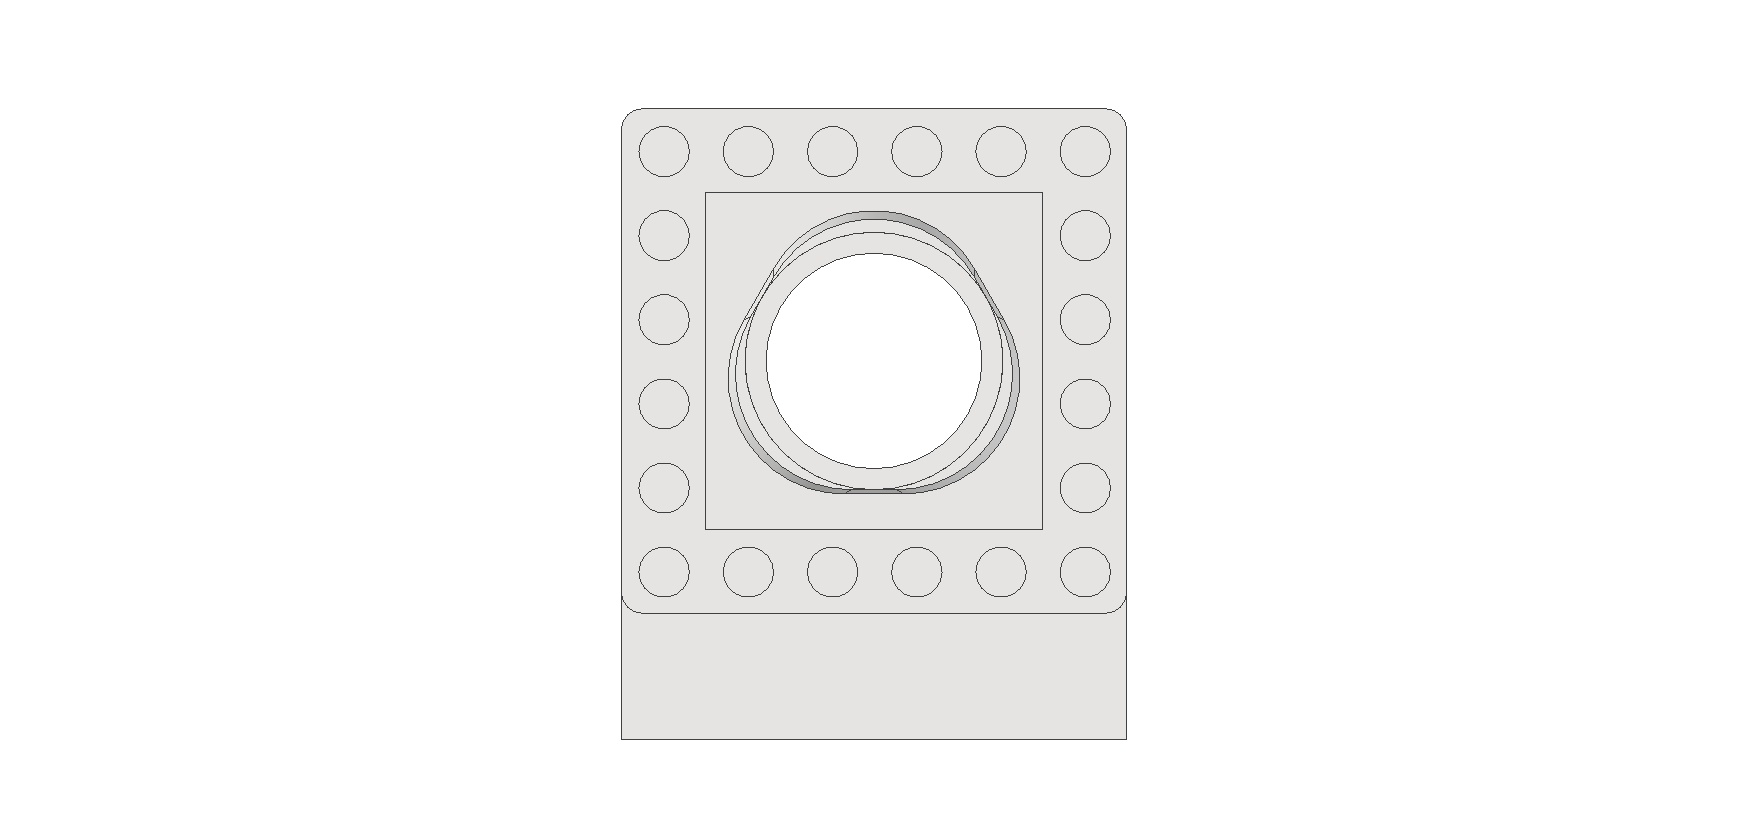
\includegraphics[width=\textwidth]{figures/ch3/fig3_29_a_Fluo_Condenser_Three_Point_Constraint.png}
        \par (a) 螢光聚光鏡 3點設計
    \end{minipage}
    \hfill
    \begin{minipage}[b]{0.48\textwidth}
        \centering
        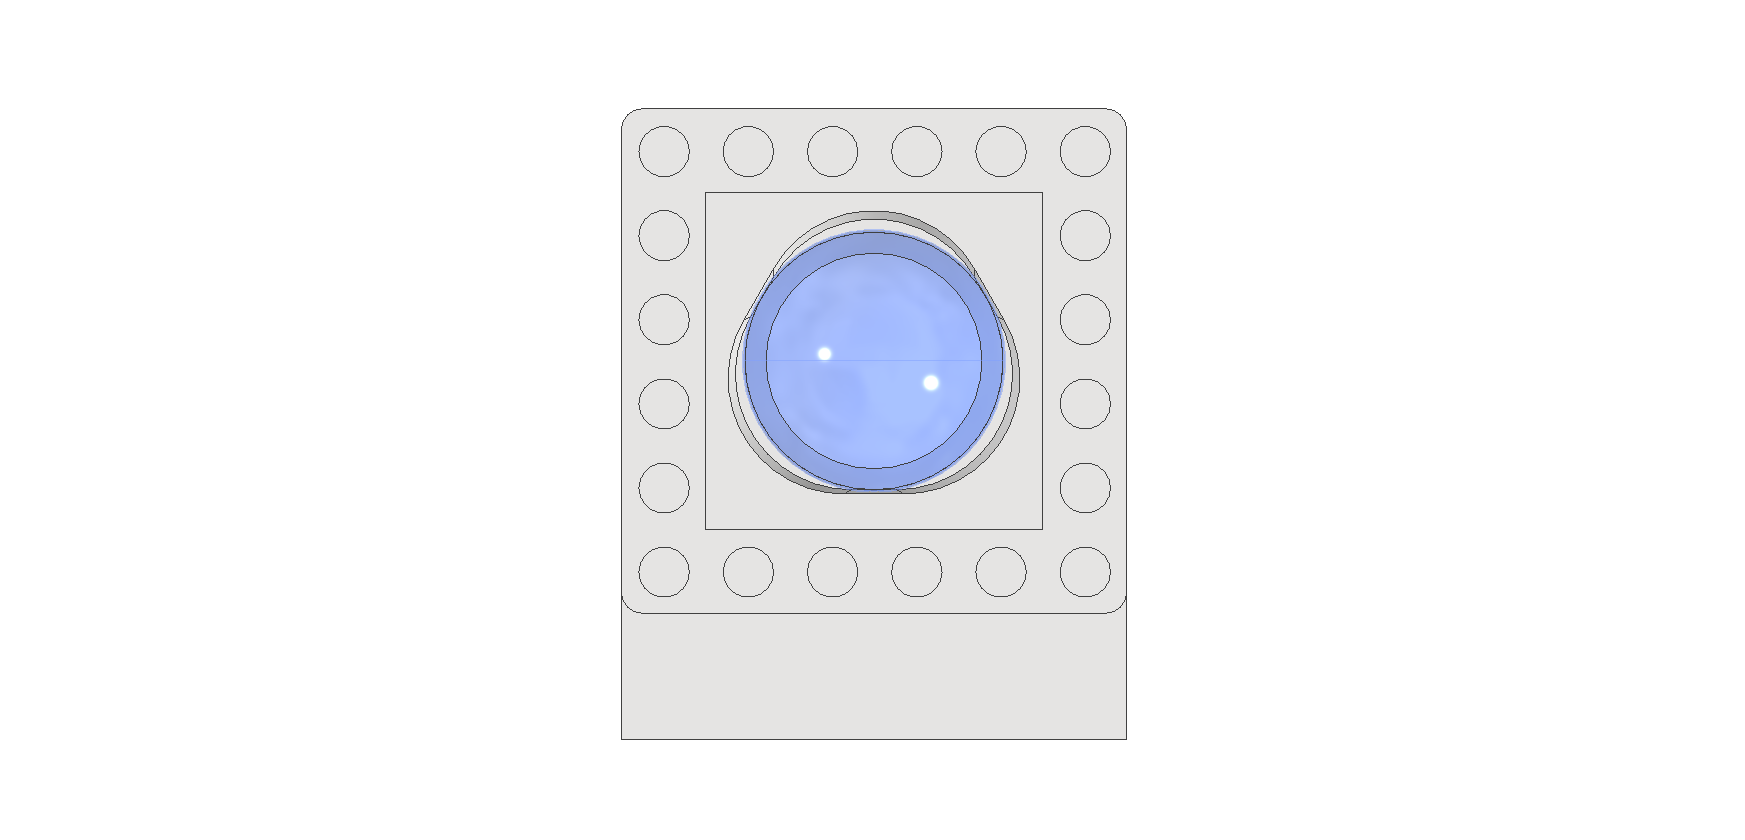
\includegraphics[width=\textwidth]{figures/ch3/fig3_29_b_Fluo_Condenser_Assembly.png}
        \par (b) 螢光聚光鏡組裝
    \end{minipage}
    \vspace{0.5cm}
    
    \begin{minipage}[b]{0.8\textwidth}
        \centering
        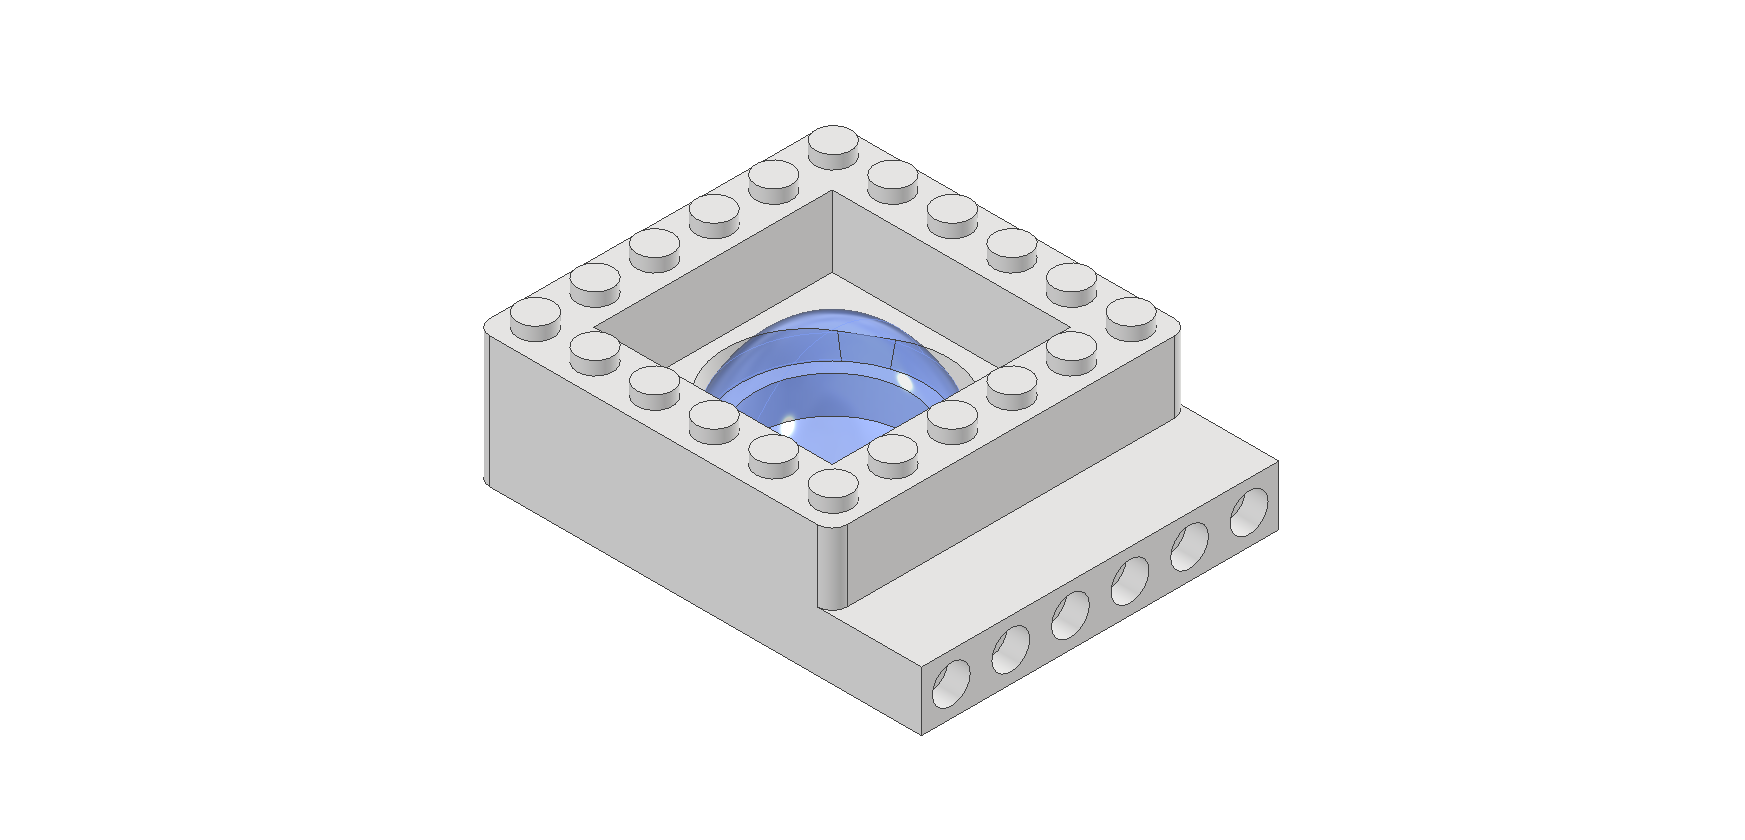
\includegraphics[width=\textwidth]{figures/ch3/fig3_29_c_Fluo_Condenser_Three_Point_3.png}
        \par (c) 45度視角的組裝
    \end{minipage}
    \caption{螢光聚光鏡之三點約束（Three-Point Constraint）支撐設計}
    \label{fig:design_3point_fluo}
\end{figure}
